\documentclass[../DoAn.tex]{subfiles}
\usepackage{booktabs}

% chèn code vào latex
\usepackage{listings}
\usepackage{lipsum}
\usepackage{courier}    % chọn font family cho  source code
\usepackage{color} % tô màu cho code
\definecolor{dkgreen}{rgb}{0,0.6,0}
\definecolor{gray}{rgb}{0.5,0.5,0.5}
\definecolor{mauve}{rgb}{0.58,0,0.82}

\lstset{frame=tb,
  basicstyle=\footnotesize\ttfamily,
  framextopmargin=50pt,frame=bottomline
  language=Python,
  aboveskip=3mm,
  belowskip=3mm,
  showstringspaces=false,
  columns=flexible,
  %basicstyle={\small\ttfamily},
  numbers=none,
  numberstyle=\tiny\color{gray},
  keywordstyle=\color{magenta},
  commentstyle=\color{dkgreen},
  stringstyle=\color{mauve},
  breaklines=true,
  breakatwhitespace=true,
  tabsize=3
}
% end chèn code vào latex

\begin{document}

\section{Tổng quan giải pháp}
\begin{figure}
\centering
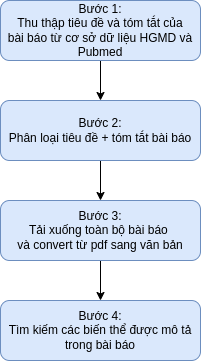
\includegraphics[width=0.6\linewidth]{Hinh_ve/soDoTongQuan_DATN.png}
\caption{Trình tự 4 bước xác định biến thể / đột biến trong bài báo khoa học}
\label{fig:3trinhtu4buoc}
\end{figure}

Để giải quyết bài toán về tự động thu thập dữ liệu, phân loại văn bản y khoa, tìm kiếm các biến thể gene được đề cập trong bài báo khoa học, em đề xuất một giải pháp gồm 4 bước như hình \ref{fig:3trinhtu4buoc}. Trong đó, \textbf{bước đầu tiên}, ta sẽ tiến hành thu thập thông tin của bài báo khoa học bao gồm tiêu đề và tóm tắt của bài báo từ 2 cơ sở dữ liệu về y tế rất uy tín là HGMD và Pubmed. \textbf{Bước số 2}, tiêu đề và bài báo được phân loại thành 2 loại, loại thứ nhất gồm những bài báo không liên quan đến bệnh ung thư, và loại số hai gồm những bài báo liên quan đến bệnh ung thư. Sau bước 2, nếu một bài báo được xác định là không liên quan đến ung thư, ta sẽ bỏ qua bài báo này và tiếp tục tìm kiêm những bài báo khác. Còn nếu ngược lại, bài toán được xác định có liên quan đến ung thư, ta sẽ chuyển qua bước 3. \textbf{Tại bước 3}, ta sẽ được tải xuống toàn bộ bài báo ở định dạng file pdf. Sau đó ta tiến hành chuyển file pdf sang dạng file txt.File txt này chứa nội dung dạng văn bản của bài báo đó (không bao gồm ảnh). \textbf{Bước 4}, ta sẽ áp dụng các biểu thức chính quy để tìm kiếm các biến thể được đề cập đến trong bài báo. Chi tiết về từng bước em có mô tả chi tiết ở những mục tiếp theo.

\section{Thu thập tiêu đề và tóm tắt của bài báo khoa học}
\subsection{Cơ sở dữ liệu HGMD The Human Gene Mutation Database - HGMD \cite{HGMD}}

\begin{figure}
\centering

\includegraphics[width=0.7\linewidth]{Hinh_ve/HGMD.png}
\caption{Logo của cơ sở dữ liệu HGMD}
\label{fig:hgmdlogo}
\end{figure}


\href{https://www.ncbi.nlm.nih.gov/pmc/articles/PMC5429360/}{HGMD} là một cơ sở dữ liệu lưu trữ những đột biến có liên quan chặt chẽ đến các bệnh di truyền ở người. Hình \ref{fig:hgmdlogo} là logo của cơ sở dữ liệu về gene người HGND. Tính đến tháng 3 năm 2017, \textbf{Hình} \ref{fig:hgmdstat} HGMD đã lưu trữ hơn 350.000 đột biến xảy ra ở trên gần 14.000 đoạn gene khác nhau. Những đột biến này đều được thu thập thủ công từ hơn 2600 bài báo khoa học. Mỗi nằm, HGMD cập nhật hơn 17000 đột biến mới được phát hiện. Dữ liệu của HGMD được các bác sĩ, nhà nghiên cứu trên toàn thế giới sử dụng để nghiên cứu, khám chữa bệnh lâm sàng tại các trung tâm chẩn đoán bệnh và tư vấn di truyền. HGMD cho phép miễn phí sử dụng dữ liệu cho các nghiên cứu học thuật .Phiên bản miễn phí bị giới hạn số lượng truy cập rất hạn chế. Nếu muốn sử dụng tài khoản miễn phí, ta có thể sử dụng email có đuôi .edu. \textbf{Hình} \ref{fig:hgmdregis} người dùng đã đăng ký phiên bản dùng thử và đợi xét duyệt từ phía quản trị viên thành công. Ngoài ra có thể sử dụng phiên bản tính phí theo bản quyền của qiagen có giá 80.000 đô la mĩ cho quyền truy cập không giới hạn các bằng chứng về gene tại HGMD trong vòng 1 năm. Cơ sở dữ liệu về đột biến gen ở người (HGMD) đại diện cho một nỗ lực đối chiếu các tổn thương gen đã biết (đã được công bố) gây ra bệnh di truyền ở người. Cơ sở dữ liệu này, trong khi ban đầu được thiết lập để nghiên cứu các cơ chế đột biến trong gen người, hiện đã có được một tiện ích rộng hơn nhiều, trong đó nó thể hiện một nguồn tham khảo cập nhật và toàn diện về phổ gen người được thừa kế thương tổn. Do đó, HGMD cung cấp thông tin có tầm quan trọng chẩn đoán thực tế cho các nhà nghiên cứu và chẩn đoán về di truyền học phân tử ở người, các bác sĩ quan tâm đến tình trạng di truyền cụ thể ở một bệnh nhân hoặc gia đình cụ thể, và các nhà tư vấn về các bệnh có di truyền từ cha mẹ sang con cái.

\begin{figure}
\centering
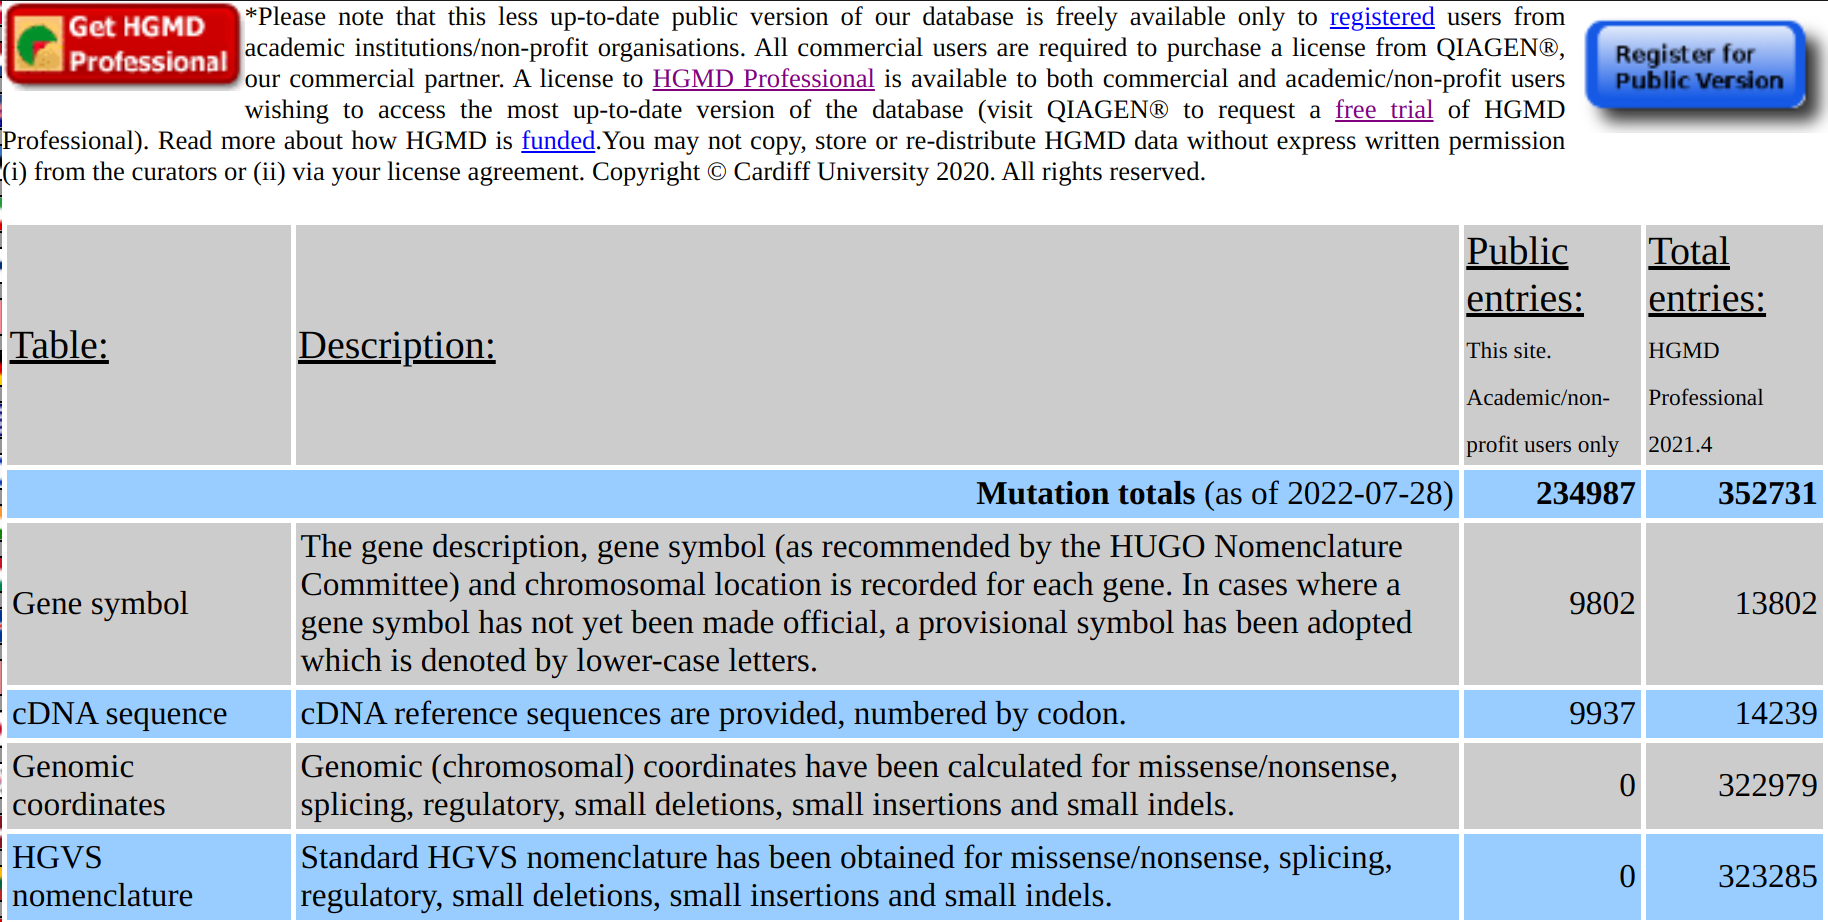
\includegraphics[width=1\linewidth]{Hinh_ve/stat_mutationHGMD.png}
\caption{Thống kê về số lượng các đột biến ở người được ghi nhận tại trang chủ của cơ sở dữ liệu HGMD, phiên phản professional cung cấp đầy đủ các đột biến hơn khi cho phép truy cập vào hơn 350.000 biến thể so với phiên phản thông thường chỉ cung cấp khoảng 235.000 biến thể, phiên bản professional cung cấp những bằng chứng mới nhất được tìm thấy, còn phiên bản thông thường chỉ có một số lượng hạn chế hơn, thông thường những bằng chứng mới nhất và đặc biệt là những biến thể hiếm sẽ được cung cấp rất hạn chế ở phiên bản thông thường}
\label{fig:hgmdstat}
\end{figure}

Cơ sở dữ liệu về đột biến gen ở người đầu tiên về tất cả các đột biến gây ra hoặc liên quan đến bệnh di truyền ở người, cộng với thường biến / liên quan đến bệnh được báo cáo trong các báo cáo khoa học. HGMD cũng bao gồm các báo cáo bổ sung cho các đột biến nhất định nếu các báo cáo này có tác dụng cải thiện việc lập mục cho các báo cáo khoa học được lưu trữ tại HGMD. Tuy nhiên cơ sở dữ liệu HGMD thường không bao gồm các đột biến mà không có mô tả rõ ràng các hậu quả có thể gây ra về kiểu hình, Ngay cả khi một số biến thể như vậy cũng đóng góp vào việc chuẩn đoán lâm sàng. Nhiều kết quả tìm kiếm đột biến đã được công bố xác định là đã gây ra bởi nhiều hơn một đột biến di truyền ở một bệnh nhân. Trong những trường hợp như vậy, mối quan hệ giữa một tổn thương nhất định và kiểu hình lâm sàng không phải lúc nào cũng rõ ràng ngay lập tức, và những người chuyên gia của HGMD đã phải hoàn toàn dựa vào đánh giá của các tác giả, người phê duyệt và biên tập viên các tạp chí nơi mà bài báo đó được đăng tải. Do đó không thể loại trừ khả năng vô tình đưa vào một số tổn thương có ít hoặc không có ý nghĩa bệnh lý. 

Các đột biến bệnh lý làm phá vỡ đột ngột cấu trúc của một gen nhất định có khả năng rất cao sẽ gây ra thay đổi kiểu hình liên quan đến gene bị đột biến đó. Tuy nhiên, đối với các loại tổn thương khác, các đột biến bệnh lý thường khó phân biệt với các dạng đa hình có ít hoặc không có ý nghĩa lâm sàng, đặc biệt nếu hậu quả về cấu trúc hoặc chức năng của chúng là nhỏ. Do đó, bằng chứng cho tính xác thực của gene gây bệnh trong bối cảnh bệnh lý thường đến từ một hoặc nhiều dòng bằng chứng khác nhau như, sự kết hợp giữa bố và mẹ gây đột biến cho con cái. Không có bất kỳ tổn thương nào khác trong gen có thể chịu trách nhiệm cho kiểu hình lâm sàng mà có thể quan sát được. hay sự xuất hiện đột ngột trên gene của một cá thể độc lập, tức trước đó không tồn tại hay ghi nhận biểu thiện từ thế hệ trước. Hoặc có thể kể đến như sự đột biến xảy ra trên protein cũng có thể gây bệnh. Có thể giả định rằng một số loại tổn thương gen được liệt kê trong HGMD có khả năng bao gồm một số đột biến không thực sự gây bệnh ngay cả khi chúng đã được báo cáo là gây ra bệnh. Việc sai sót này có thể do nhiều nguyên nhân khác nhau, có thể do tác giả của bài báo hoặc cũng có thể nguyên nhân gây ra là do sự nhầm lẫn của các chuyên gia tại HGMD. Vì vậy, người sử dụng HGMD nên biết rằng, hiện tại, HGMD không có phương tiện hoàn toàn khách quan nào để biết chính xác mức độ gây bệnh của từng loại đột biến về mặt xác thực bệnh lý của các tổn thương được liệt kê trong đó. Tuy nhiên, các nghiên cứu gần đây đã cung cấp bằng chứng rằng phần lớn các alen hiếm cũng có khả năng gây hại. 

\begin{figure}
\centering
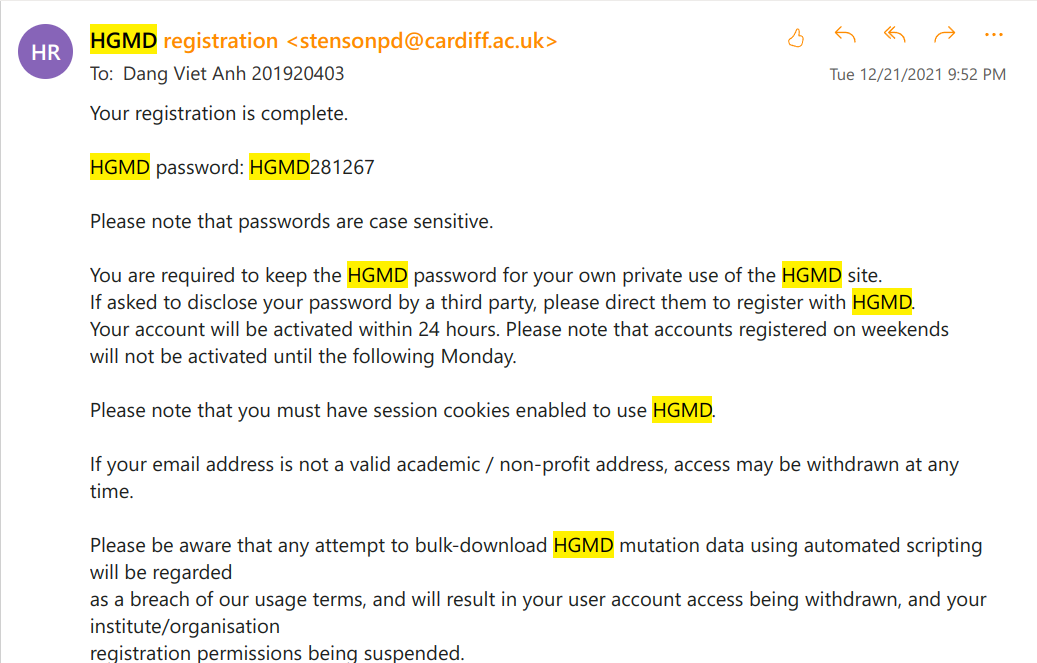
\includegraphics[width=1.05\linewidth]{Hinh_ve/HGMD_register.png}
\caption{Email đăng ký sử dụng HGMD thành công được gửi từ phía quản trị viên của cơ sở dữ liệu HGMD}
\label{fig:hgmdregis}
\end{figure}

\begin{figure}
\centering
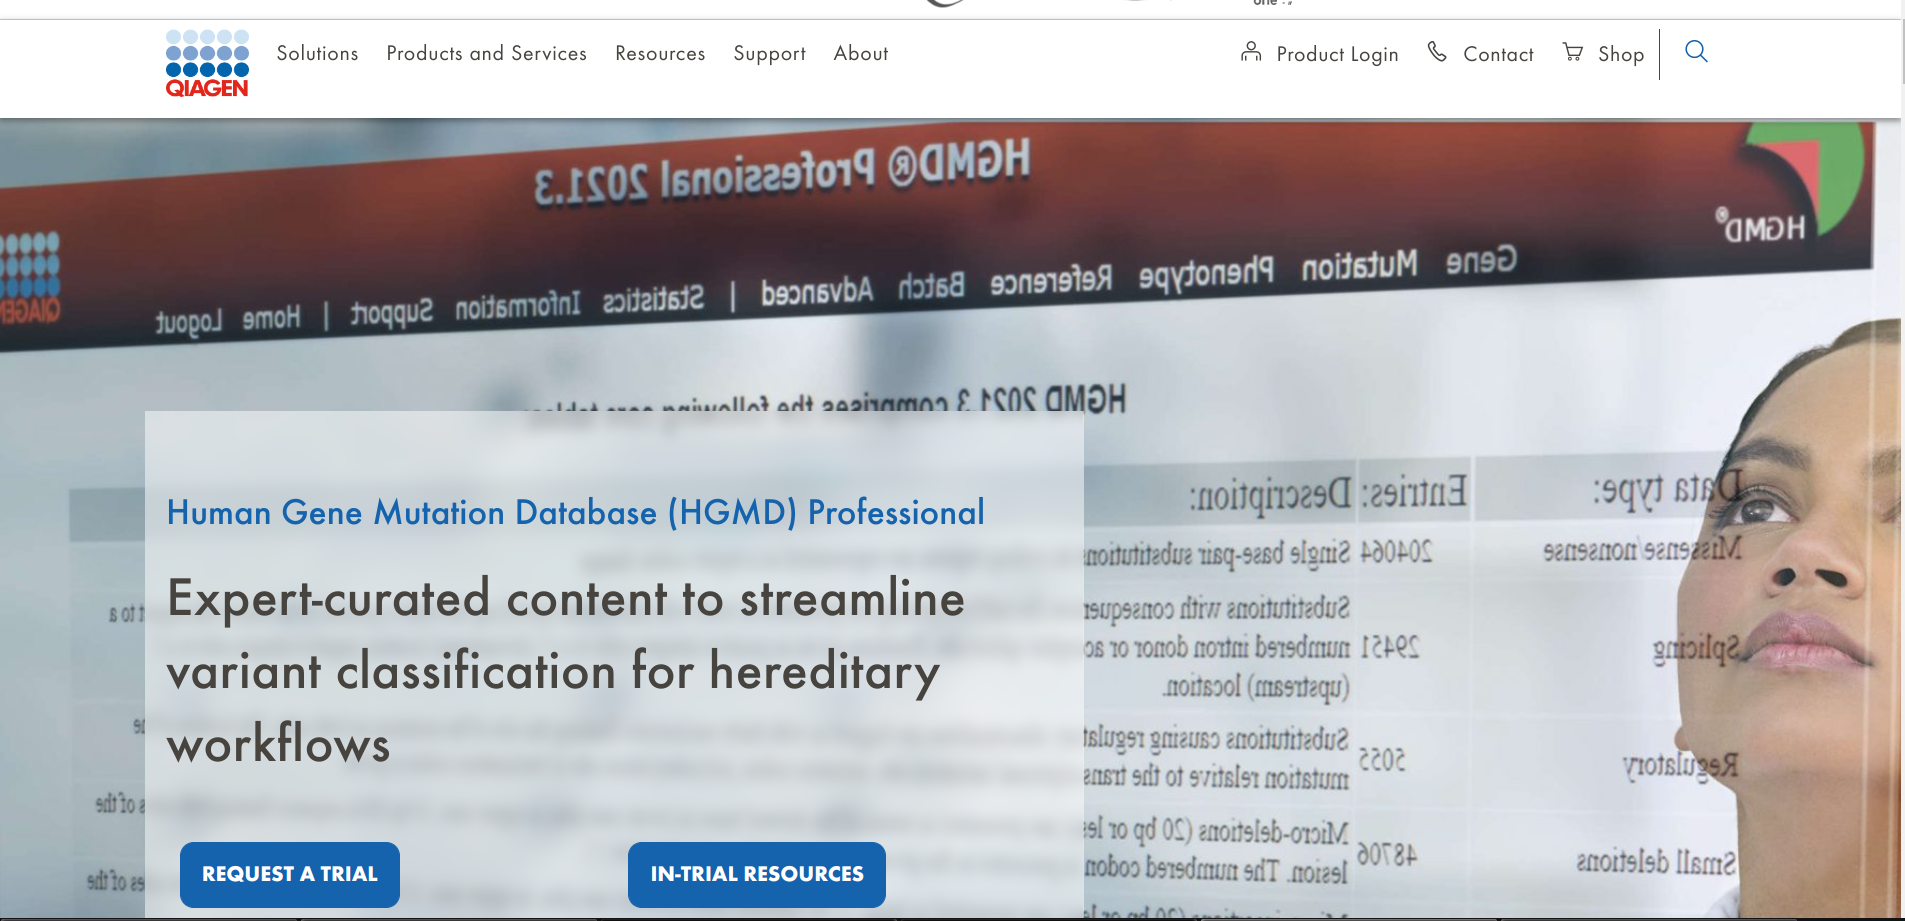
\includegraphics[width=1\linewidth]{Hinh_ve/HGMDpro.png}
\caption{Giao diện của HGMD Professional}
\label{fig:hgmdpro}
\end{figure}


\begin{figure}
\centering

\includegraphics[width=1\linewidth]{Hinh_ve/Pubmed_logologo.png}
\caption{logo của cơ sở dữ liệu Pubmed}
\label{fig:pubmedlogo}
\end{figure}


\subsection{Cơ sở dữ liệu Pubmed}
Pubmed là cơ sở dữ liệu lưu trữ tiêu đề và tóm tắt về các bài báo về y sinh, hóa học, sinh học. \textbf{Hình} \ref{fig:pubmedlogo} Mỗi một bài báo tại đây đều có một định danh duy nhất được gọi là PMID (pubmed identifier number). Mỗi bài báo được lưu trữ tại đây đều được pubmed lưu trữ rất đầy đủ tiêu đề, tóm tắt, và các thông tin trích dẫn cũng như tài liệu tham khảo của paper đó. Tuy nhiên, pubmed chỉ lưu trữ một phần toàn văn của bài báo đó. Mỗi trường thông tin trên đều được sử dụng cho mục đích để thu thập dữ liệu riêng. Trong đó, PMID dùng để định dạnh một bài báo duy nhất được xác định trên cơ sở dữ liệu Pubmed. Tiêu đề và tóm tắt có thể được thu thập cho bài toán phân loại văn bản. Chính tiêu đề và tóm tắt sẽ là dữ liệu để huấn luyện mô hình phân loại văn bản ở những bước sau. Tuy nhiên, những bài báo tạo pubmed sẽ có đầy đủ các tiêu đề, nhưng một số lượng lớn các bài báo lại không có tóm tắt nguyên nhân do tác giả của bài báo đó không viết phần tóm tắt này. Ngoài ra, danh sách tài liệu tham khảo, danh sách bài báo trích dẫn và danh sách bài báo tương tự được cơ sở dữ liệu Pubmed gợi ý đều được dùng để tìm kiếm các bài báo có liên quan. Những danh sách này sẽ được dùng để tự động thu thập dữ liệu chỉ xuất phát với ban đầu là duy nhất một PMID, việc này sẽ giúp tránh được việc xác định một số lượng lớn các PMID biết trước khi tiến hành thu thập dữ liệu. Vì cơ sở dữ liệu Pubmed không lưu trữ tất cả các bài báo toàn văn, vì thế, chỉ số DOI sẽ được sử dụng để tìm kiếm và xác định bài báo đó trên Scihub, nhằm mục đích tải về toàn bộ bài báo khoa học, sử dụng để tìm kiếm biến thể đột biến. \textbf{Hình} \ref{fig:3pubmedpaper} , \textbf{hình} \ref{fig:3pubmedpaper2} và \textbf{hình} \ref{fig:3pubmedpaper3} hiển thị các trường thông tin của bài báo khoa học đăng tại Pubmed. Trong đó số 1 là tiêu đề của bài báo khoa học. Số 2 là tóm tắt của bài báo đó, mục số 2 này có thể không có ở một số lượng lớn các bài báo. Số 3 là danh sách các bài báo liên quan đến bài báo đang xem xét, danh sách bài báo tương tự được Pubmed gợi ý. SỐ 4 là chỉ số DOI của bài báo, chỉ số này có ích rất lớn trong việc xác định bài báo trên internet. Chỉ số này còn có thể sử dụng để tìm kiếm, tra cứu, tải xuống bài báo ở trên Scihub. Số 5 chính là PMID (pubmed identifier number), số này dùng để định danh bài báo trên cơ sở dữ liệu của Pubmed, và số này là duy nhất. Đại diện cho một bài báo tại cơ sở dữ liệu này. Hình \ref{fig:3pubmedpaper2}: Số 6 là danh sách những bài báo trích dẫn. Hình \ref{fig:3pubmedpaper3}: Số 7 là danh sách những bài báo tham khảo.

\begin{figure}
\centering
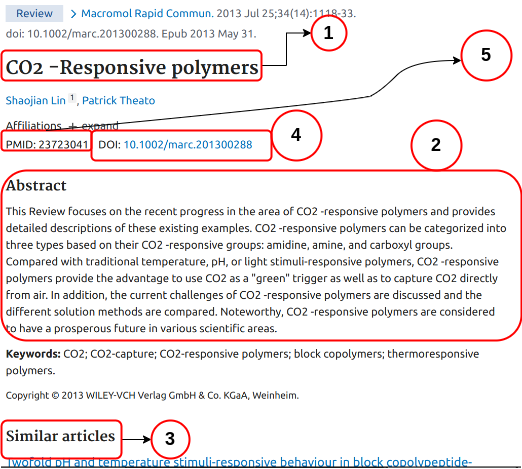
\includegraphics[width=1.0\linewidth]{Hinh_ve/PubmedPaper.png}
\caption{Các trường thông tin quan trọng cần thu thập về một bài báo khoa học của trên cơ sở dữ liệu Pubmed. Trong đó số 1 là tiêu đề của bài báo khoa học. Số 2 là tóm tắt của bài báo đó, mục số 2 này có thể không có ở một số lượng lớn các bài báo. Số 3 là danh sách các bài báo liên quan đến bài báo đang xem xét, danh sách bài báo tương tự được Pubmed gợi ý. SỐ 4 là chỉ số DOI của bài báo, chỉ số này có ích rất lớn trong việc xác định bài báo trên internet. Chỉ số này còn có thể sử dụng để tìm kiếm, tra cứu, tải xuống bài báo ở trên Scihub. Số 5 chính là PMID (pubmed identifier number), số này dùng để định danh bài báo trên cơ sở dữ liệu của Pubmed, và số này là duy nhất. Các thông tin khác xem hình \ref{fig:3pubmedpaper2} và \ref{fig:3pubmedpaper3}. }
\label{fig:3pubmedpaper}
\end{figure}

\begin{figure}
\centering
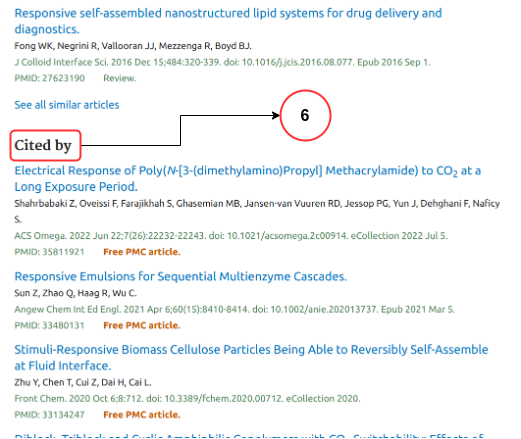
\includegraphics[width=1.0\linewidth]{Hinh_ve/Pubmedpaper2.png}
\caption{Các trường thông cần quan tâm về một bài báo khoa học của trên cơ sở dữ liệu Pubmed. Trong đó, số 6 là danh sách những bài báo trích dẫn. Các thông tin khác xem hình \ref{fig:3pubmedpaper} và hình \ref{fig:3pubmedpaper3}.}
\label{fig:3pubmedpaper2}
\end{figure}

\begin{figure}
\centering
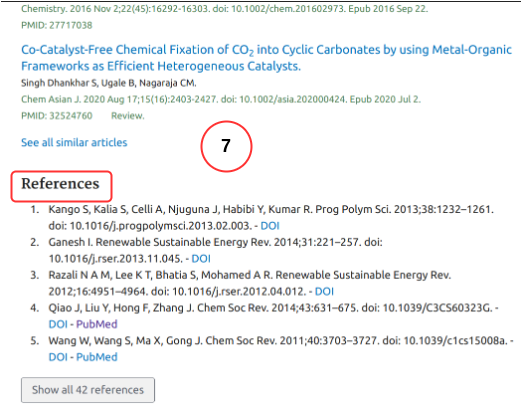
\includegraphics[width=1.0\linewidth]{Hinh_ve/PubmedPaper3.png}
\caption{Các trường thông cần quan tâm về một bài báo khoa học của trên cơ sở dữ liệu Pubmed. Trong đó, số 7 là danh sách các bài báo tham khảo. Các trường thông tin khác xem hình \ref{fig:3pubmedpaper} và hình \ref{fig:3pubmedpaper2}. }
\label{fig:3pubmedpaper3}
\end{figure}

\subsection{Cơ sở dữ liệu Pubmed Central}
\begin{figure}
\centering
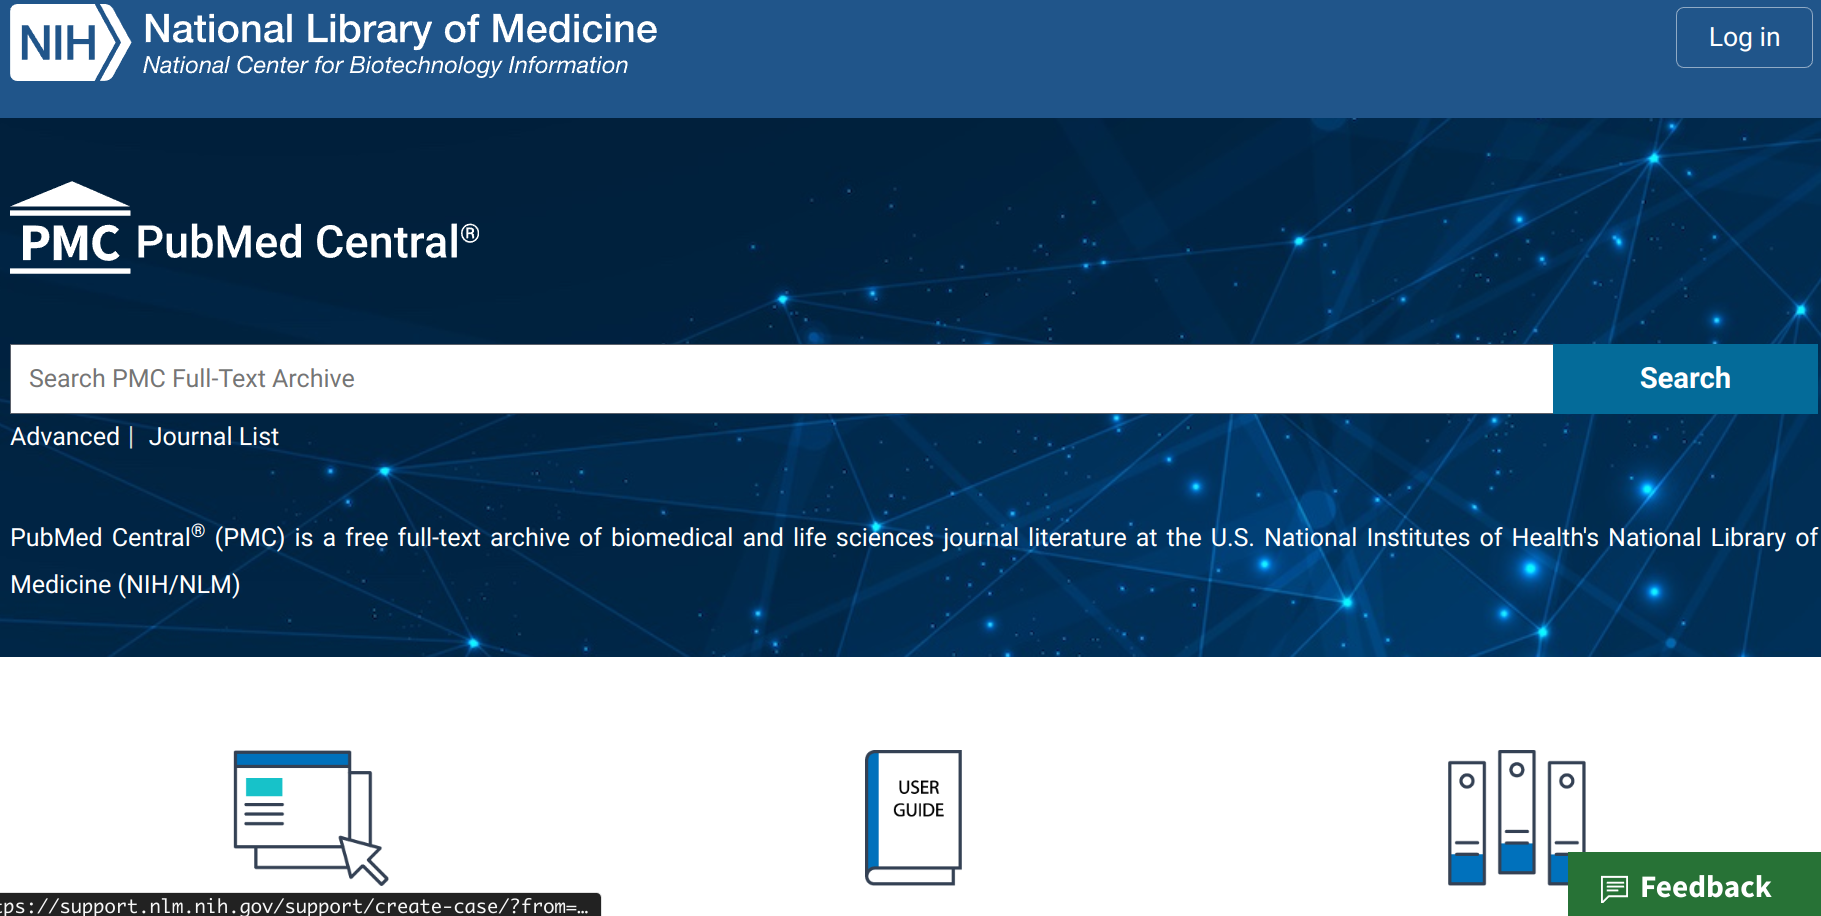
\includegraphics[width=1.0\linewidth]{Hinh_ve/PMCHomepage.png}
\caption{Trang chủ của cơ sở dữ liệu Pubmed Central - PMC có địa chỉ tại ``https://www.ncbi.nlm.nih.gov/pmc/``. PubMed Central® (PMC) là một kho lưu trữ toàn bộ bài báo khoa học miễn phí được tổng hợp từ các tài liệu tạp chí y sinh và khoa học đời sống tại Thư viện Y khoa Quốc gia của Viện Y tế Quốc gia Hoa Kỳ (NIH / NLM)}
\label{fig:PMChomepage}
\end{figure}

PubMed Central® (PMC) hình \ref{fig:PMChomepage} là một kho lưu trữ toàn văn miễn phí các tài liệu tạp chí khoa học đời sống và y sinh tại Thư viện Y khoa Quốc gia của Viện Y tế Quốc gia Hoa Kỳ (NIH / NLM). Pubmed Central có địa chỉ chính thức tại ``https://www.ncbi.nlm.nih.gov/pmc/`` .Ngoài ra, Pubmed Central cũng cung cấp một địa chỉ để có thể tải về toàn bộ cơ sở dữ liệu của Pubmed Central tại ``https://ftp.ncbi.nlm.nih.gov/``. Cơ sở dữ liệu cũng cho phép thu thập dữ liệu tự động thông qua các API được cung cấp bởi chính Pubmed Central. Để phù hợp với nhiệm vụ lập pháp của NLM trong việc thu thập và bảo quản các tài liệu y sinh, PMC là một phần của bộ sưu tập NLM, cũng bao gồm bản in rộng rãi và các tạp chí điện tử được cấp phép của NLM, đồng thời hỗ trợ nghiên cứu và thực hành y sinh và chăm sóc sức khỏe đương đại cũng như học bổng trong tương lai. Pubmed Central cho phép công chúng truy cập trực tuyến kể từ năm 2000, Pubmed Central-PMC được phát triển và được duy trì bởi Trung tâm Thông tin Công nghệ Sinh học Quốc gia (NCBI) tại NLM. Kể từ khi thành lập vào năm 2000, PMC đã phát triển từ chỗ chỉ bao gồm hai tạp chí, PNAS: Kỷ yếu của Viện Hàn lâm Khoa học Quốc gia và Sinh học Phân tử của Tế bào, thành một kho lưu trữ các bài báo từ hàng nghìn tạp chí. Ngày nay, PMC chứa hơn 7 triệu bài báo khoa học toàn văn, trải qua nhiều thế kỷ nghiên cứu y sinh và khoa học đời sống (cuối những năm 1700 đến nay). Nội dung được thêm vào kho lưu trữ thông qua nhiều nguồn, ví dụ như các nhà xuất bản, hiệp hội học thuật và chủ sở hữu nội dung khác để gửi các bài báo tạp chí trực tiếp cho PMC. Ngoài ra , PMC cũng có tài trợ cho các nghiên cứu khoa học, chính vì thế, PMC có thể tiếp cận các bài báo này, ngay từ khi các bài báo mới chỉ ở dạng bản thảo. Ngoài ra PMC cũng lưu trữ các bài báo khoa học đã cữ dưới dạng bản scan, việc thu thập các báo cáo đã cũ được thu thập thông qua việc rà soát các tạp chí khoa học để tìm kiếm, để chuyển đổi từ bản scan qua dạng văn bản, PMC có sử dụng công nghệ nhận diện ký tự quang học (Optical character recognition- OCR). Tuy nhiên, PMC không phải là nhà xuất bản của các bài báo khoa học, kết quả của việc thu thập và lưu trữ những báo cáo khoa học tại đây là do sự hợp tác với các nhà xuất bản, tài trợ cho các nghiên cứu khoa học và rà soát bài báo từ các tạp chí cũ.

Pubmed Central có trách nhiệm bảo quản vĩnh viễn các báo cáo khoa học về các lĩnh vực có liên quan đến y học. Tất cả các nội dung tại PMC đều là miễn phí để đọc (trừ các trường hợp đặc biệt như bị cấm vận, ...), vì NLM tin rằng cách tốt nhất để đảm bảo khả năng truy cập và khả năng tồn tại của tài liệu kỹ thuật số theo thời gian là sử dụng nhất quán và tích cực kho lưu trữ. Tuy nhiên, truy cập miễn phí không có nghĩa là không được bảo vệ bản quyền của nội dung đó. 

PMC lưu trữ nội dung bằng ngôn ngữ đánh dấu eXtensible (XML), thể hiện cấu trúc và ý nghĩa của tài liệu ở dạng tương đối đơn giản và con người có thể đọc được. Tất cả nội dung tại PMC đều được chuyển đổi sang và lưu trữ ở định dạng NISO Z39.96-2015 JATS XML. Định dạng tiêu chuẩn này là định dạng lưu trữ hiệu quả nhất và được sử dụng rộng rãi cho các bài báo trên các tạp chí khoa học.

NLM vận hành mạng lưới PMC International, mạng này cung cấp một khuôn khổ để duy trì các bản sao của kho tài liệu PMC trong các kho lưu trữ quốc tế đáng tin cậy khác có chung mục tiêu của PMC và hoạt động theo các nguyên tắc giống nhau.

Bởi vì Pubmed Central - PMC có khả năng lưu trữ các trích dẫn chéo từ các nguồn khác nhau theo một định dạng chung trong một kho lưu trữ trung tâm, người dùng PMC có thể nhanh chóng tìm kiếm toàn bộ bộ sưu tập các bài báo toàn văn và tìm tất cả các tài liệu có liên quan. Cấu trúc của kho lưu trữ PMC cũng hỗ trợ tích hợp tài liệu với các tài nguyên khác.

PMC cho phép truy xuất hàng loạt các file phục vụ cho mục đích trích xuất văn bản và các mục đích khác trong một số bộ sưu tập hoặc tập hợp con của kho lưu trữ PMC.

Ngoài việc đảm bảo bảo quản lâu dài các tài liệu khoa học, PMC cung cấp quyền truy cập vào kho lưu trữ ở các định dạng có thể đọc được dễ dàng bằng máy tính hoặc truy cập thủ công bởi con người. Việc sử dụng PMC đã tăng lên khi kho lưu trữ đã phát triển. Các con số được báo cáo tại bảng \ref{tab:statPMCrequest} phản ánh quyền truy cập vào trang web PMC trong tháng cuối cùng của mỗi năm tài chính (tức là vào tháng 9). Có thể dễ dàng thấy rằng, số lượng bài báo và số lượng truy cập tăng nhanh sau mỗi năm, đặc biệt là từ 2019 sang 2020, khi mà đại dịch Covid-19 lây lan khắp các quốc gia trên thế giới.

Có thể thấy rằng, Pubmed và Pubmed Central là hai cơ sở dữ liệu lưu trữ những thông tin có phần khác nhau. Khi mà Pubmed chỉ lưu trữ thông tin về một bài báo như tiêu đề, tóm tắt, danh sách các bài báo tham khảo, danh sách các bài báo trích dẫn ,... thì Pubmed Central lại lưu trữ đầy đủ toàn bộ bài báo và cho phép truy cập miễn phí và không giới hạn bởi cả cách thủ công lẫn bằng các công cụ thu thập dữ liệu. 

\begin{table}[]
\caption{Thống kê số lượng bài báo khoa học được lưu trữ và cho phép truy cập miễn phí tại Pubmed Central. Và số lượng truy cập trung bình mỗi tuần. Có thể thấy rằng, số lượng các bài báo và số lượng truy cập tăng nhanh theo mỗi năm. Đặc biệt là từ 2019 sang 2020, khi mà đại dịch Covid-19 lây lan khắp các quốc gia trên thế giới.}
\label{tab:statPMCrequest}
\begin{tabular}{@{}ccc@{}}
\toprule
\textbf{Năm tài chính} & \textbf{Số lượng bài báo tại PMC} & \textbf{Lượng truy cập tính theo tuần} \\ \midrule
2021 & 7,383,455 & 3.1 triệu \\
2020 & 6,471,176 & 3.4 triệu \\
2019 & 5,725,819 & 2.6 triệu \\
2018 & 5,107,590 & 2.4 triệu \\
2017 & 4,553,343 & 2.1 triệu \\
2016 & 4,054,283 & 1.3 triệu \\
2015 & 3,623,566 & 1.2 triệu \\
2014 & 3,227,379 & 886,000   \\
2013 & 2,859,268 & 834,000   \\ \bottomrule
\end{tabular}
\end{table}



\subsection{Mô tả công cụ thu thập dữ liệu từ pubmed}
\begin{figure}
\centering

\includegraphics[width=1.\linewidth]{Hinh_ve/requestPubmed.png}
\caption{Địa chỉ của một bài báo tại cơ sở dữ liệu Pubmed. Trong đó, ô màu đỏ bên trái là địa chỉ trang chủ của Pubmed, ô màu đỏ bên phải là chỉ số PMID của bài báo đó. Nếu đã biết chỉ số PMID và muốn truy cập vào bài báo đó, ta chỉ có thể thay thế PMID vào đường dẫn và gửi request, ta có thể làm việc này bằng cách sửa địa chỉ trực tiếp trên trình duyệt. Ví dụ ta muốn truy cập bài báo có số PMID là \textbf{12345678}, ta chỉ cần gửi request có nội dung ``https://pubmed.ncbi.nlm.nih.gov/\textbf{12345678}/``}
\label{fig:reqPubmed}
\end{figure}
Để thu thập được một lượng lớn dữ liệu thì việc cần một công cụ hỗ trợ là việc rất cần thiết. Toàn bộ chương trình thu thập dữ liệu em đã lưu tại địa chỉ \begin{verbatim} https://tinyurl.com/33vhsb59 \end{verbatim}. Cụ thể cách hoạt động của chương trình được mô tả \ref{fig:crawPubmed}.
Vì phương thức truy xuất dữ liệu của Pubmed được thiết kế ở phương thức GET, vì thế, ta có thể dễ dàng nhìn thấy cách gửi request từ trình duyệt đến servert của Pubmed \ref{fig:reqPubmed} như hình gồm 2 thành phần. phần khoanh màu bên trái là đường dẫn cố định, còn phần bên phải chính là PMID của bài báo khoa học mình cần tìm. Chính vì thế, em đã đề xuất xây dựng công cụ thu thập dữ liệu gồm 4 bước như \textbf{hình} \ref{fig:crawPubmed}. Ở \textbf{bước 1}, ta  chỉ cần gửi request theo phương thức GET đến địa chỉ cho trước, ta sẽ nhận được phản hồi là thông tin bài báo ta cần. Phía dưới là một hàm gửi một request đến Pubmed.
\begin{lstlisting}
def send_request(url: str, headers) -> Tag:
    resp = requests.get(url, headers, timeout=5)
    soup = BeautifulSoup(resp.text, "lxml")
    return soup.find('body')
\end{lstlisting}


\textbf{Bước 2} thông tin phản hồi này sẽ bao gồm đầy đủ các thông tin như tên tiêu đề, tóm tắt, chỉ số DOI, danh sách bài báo tham khảo, danh sách bài báo trích dẫn, danh sách bài liên quan được Pubmed gợi ý. Tất cả các thông tin này đều quan trọng trong việc thu thập dữ liệu và sẽ được sử dụng trong nhiều mục đích khác nhau.

\textbf{Bước 3} Từ phản hồi nhận được, ta tiến hành phân tích dữ liệu ở bên trong file html để tìm kiếm các trường thông tin. Phía dưới là hàm để tìm kiếm thông tin về tiêu đề của bài báo.
\begin{lstlisting}
def find_title(body: Tag) -> str:
    tit=body.find(name='h1',{'class':'heading-title'})
    tit= tit.get_text(strip=True)
    return ' '.join(tit.split())
\end{lstlisting}

Tìm kiếm thông tin về tóm tắt của bài báo bằng cách sử dụng hàm bên dưới. Đây là dữ liệu quan trọng dùng để huấn luyện mô hình xây dựng văn bản. Tại Pubmed, tồn tại một số lượng đáng kể các bài báo không có tóm tắt. Đối với những trường hợp không có tóm tắt này, hàm sẽ trả về một chuỗi ký tự rỗng.
\begin{lstlisting}
def find_abstract(body: Tag) -> str:
    absTag = body.find(name='div',
                      {"class":"abstract"},
                       recursive=True)
    if absTag is not None:
        _abstract = absTag.find('p')
        if _abstract is None:
            return ""
        else:
            return _abstract.get_text()
\end{lstlisting}

Tìm kiếm danh sách bài báo tham khảo bằng cách sử dụng hàm bên dưới. Danh sách bài báo tham khảo được sử dụng để tìm kiếm các bài báo liên quan khác trong trường hợp chưa xác định trước được chỉ số PMID.
\begin{lstlisting}
def find_reference_body(body: Tag) -> Tag:
    ref=body.find('button',
        {"aria-controls":"top-references-list-1",
         "class":"show-all",
         "data-ga-action":"show_more",
         "data-ga-category":"reference"},
         recursive=True)
    nPage=ref.__getitem__(key='data-next-page-url')
    return send_request(urljoin(PUBMED, nPage))
\end{lstlisting}

Tìm kiếm danh sách bài báo tương tự được Pubmed gợi ý bằng hàm bên dưới, danh sách bài báo tương tự được sử dụng như là những bài báo có liên quan đến bệnh ung thư. Danh sách này được sử dụng làm lớp dữ liệu dương tính (positive) khi tiến hành huấn luyện mô hình phân loại văn bản.
\begin{lstlisting}
def find_similar_body(body: Tag)->Tag:
    similarTag=body.find('a',
        {'class':'usa-button show-all-linked-articles', 
         "data-ga-action":"show_all", 
         "data-ga-category":"similar_article"},
         recursive=True)
    query=similarTag.__getitem__(key='data-href')
    return send_request(add_query(query))
\end{lstlisting}

Tìm kiếm danh sách bài báo trích dẫn bằng hàm bên dưới. Danh sách bài báo trích dẫn được sử dụng để tìm kiếm các bài báo liên quan khác trong trường hợp chưa xác định trước được chỉ số PMID.
\begin{lstlisting}
def find_cited_body(body: Tag)->Tag:
    cited = body.find('a',
        {"class":"usa-button show-all-linked-articles",
         "data-ga-category":"cited_by", 
         "data-ga-action":"show_all"},recursive=True)
    query=cited.__getitem__(key="data-href")
    return send_request(add_query(query))
\end{lstlisting}

Tìm kiếm chỉ số DOI của bài báo bằng hàm bên dưới, chỉ số DOI được sử dụng để tìm kiếm toàn bộ bài báo trên Scihub:
\begin{lstlisting}
def find_DOI(body:Tag) -> str:
    doi_Tag = body.find("a",
        {"class": "id-link",
        "data-ga-action": "DOI",
        "data-ga-category":"full_text",
        "rel": "noopener",
        "target": "_blank"}, recursiv = True)
    if doi_Tag is None: return ""
    else: return doi_Tag.get_text(strip=True)
\end{lstlisting}

\textbf{Bước 4} Sau khi thu thập được các thông tin cần thiết, ta lưu trữ lại để sử dụng. Trong đó, thông tin về tiêu đề và tóm tắt sẽ được dùng cho huấn luyện mô hình phân loại văn bản. chỉ số DOI lưu trữ để tải về bài báo toàn văn nếu bài báo đó được phân loại là có liên quan đến bệnh ung thư. Các danh sách bài báo tham khảo, bài báo trích dẫn, bài báo liên quan sẽ được dùng để tìm kiếm thêm các bài báo khác khi cần thu thập thêm bài báo khoa học.

\begin{figure}
\centering
% chỉnh tỉ lệ ảnh để kéo giãn ra chiếm hết 1 trang.
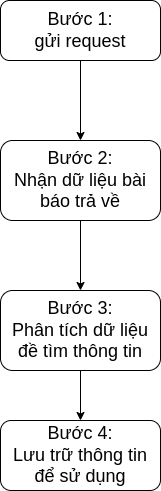
\includegraphics[width=0.35\linewidth]{Hinh_ve/craw.png}
\caption{Quy trình làm việc của công cụ thu thập dữ liệu từ Pubmed gồm 4 bước. Bước 1: thực thiện gửi request đến máy chủ của Pubmed. Bước 2: nhận thông tin phản hồi. Bước 3: phân thích thông tin trong html nhận được để nhận các trường thông tin về bài báo khoa học. Bước 4: Lưu trữ các trường thông tin về bài báo khoa học.}
\label{fig:crawPubmed}
\end{figure}



\begin{figure}
\centering
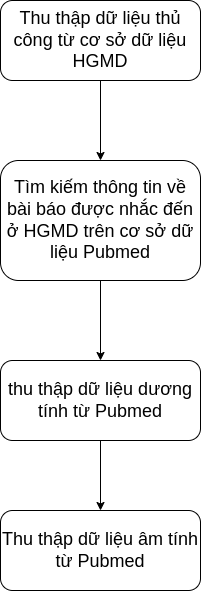
\includegraphics[width=0.4\linewidth]{Hinh_ve/thuthapdulieu.png}
\caption{Quy trình thu thập dữ liệu cho bài toán phân loại tiêu đề và tóm tắt giữa bài báo liên quan đến gene và không liên quan đến gene. Bước 1 thu thập dữ liệu thủ công từ cơ sở dữ liệu HGMD, dữ liệu thu thập từ HGMD sẽ được gán nhãn là dương tính. Bước 2: thu thập dữ liệu từ Pubmed, dữ liệu này cũng được gán nhãn là dương tính. Bước 3: thu thập dữ liệu từ cơ sở dữ liệu Pubmed Central. Dữ liệu thu thập từ Pubmed Central được gán nhãn là âm tính.}
\label{fig:thuthaphgmdpubmed}
\end{figure}
\subsection{Tiến hành thu thập thông tin về tiêu đề và tóm tắt của bài báo}
\begin{figure}
\centering
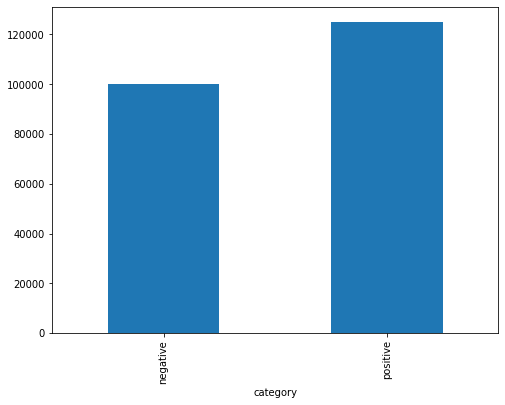
\includegraphics[width=1\linewidth]{Hinh_ve/Chuong3_dataCls.png}
\caption{Thống kê số lượng dữ liệu ở mỗi lớp. Lớp ấm tính có 100.299 dữ liệu, lớp dương tính có 124.850 dữ liệu, Tổng cộng bộ dữ liệu thu thập được gồm có 225149 dữ liệu}
\label{fig:3cls}
\end{figure}


Vì pubmed lưu trữ dữ liệu ở nhiều lĩnh vực khác nhau. Chỉ một phần nhỏ các bài báo tại đây là có liên quan đến các bệnh đột biến gây ung thư. Chính vì vậy, em đã tiến hành xây dựng một mô hình phân loại văn bản. Mô hình sẽ phân loại văn bản thành 2 loại. Loại 1 bao gồm những bài báo liên quan đến ung thư, được gọi là positive, và loại 2 bao gồm những bài báo không liên quan đến ung thư. Đẻ gán nhãn được một số lượng lớn data về chuyên ngành y sinh là điều đòi hỏi vô cùng nhiều công sức. Trong khi đó, để xây dựng một mô hình phân loại tốt phải yêu cầu một bộ dữ liệu chất lượng cao. Chính vì thế yêu cầu về thu thập dữ liệu đã được gán nhãn phải được ưu tiên hàng đầu. Để giải quyết được vấn đề này, em đã tiến hành xây dựng bộ dữ liệu văn bản về gen gây bệnh như 
Bộ dữ liệu được thu thập theo sơ đồ \textbf{hình} \ref{fig:thuthaphgmdpubmed}

Bước 1, thu thập dữ liệu thủ công từ cơ sở dữ liệu HGMD, HGMD là cơ sở dữ liệu về gene di truyền và đột biến rất lớn. Tất cả các dữ liệu tại HGMD đều được xử lý thủ công bởi các chuyên gia. Vì thế những bài báo tại đây đều đã được xác nhận là có liên quan đến ung thư. Vì thế, em đã đăng ký tài khoản dùng thử tại đây bằng email của trường \ref{fig:hgmdregis} . Tại HGMD em tìm kiếm các PMID bằng cách tìm từ khóa là các tên một đoạn gene ví dụ ABL1 , HGMD sẽ đưa ra tất cả danh sách các bài báo tương liên quan đến loại gene này. Sau đó em đã lưu file html của kết quả trả về trên trình duyệt như \textbf{hình} \ref{fig:HGMDABL1}. Từ file html này, em đã truy suất được các PMID (định danh bài báo khoa học trên cơ sở dữ liệu Pubmed). Vì lý do giới hạn số lượng request truy cập cho tài khoản dùng thử, em chỉ thu thập được 4079 PMID từ HGMD.

Bước 2, từ những PMID này em tìm kiếm những bài báo đó ở cơ sở dữ liệu Pubmed, em đã thu được thông tin về 4079 bài báo. thông tin về những bài báo này đầy đủ về tiêu đề, chỉ số DOI, danh sách các bài báo liên quan được Pubmed gợi ý, danh sách bài báo trích dẫn và danh sách tài liệu tham khảo.

Bước 3: từ 4079 bài báo đã được xác nhận là có liên quan đến gene lấy từ cơ sở dữ liệu HGMD, em tìm kiếm những bài báo nằm trong danh sách bài báo có liên quan được cơ sở dữ liệu Pubmed gợi ý. Kết quả, em đã thu thập được thêm 124.850 bài báo. Bài báo này và 4079 bài báo lấy từ HGMD tạo thanh bộ dữ liệu dương tính (positive) cho bài toán phân loại văn bản.

\begin{figure}
\centering
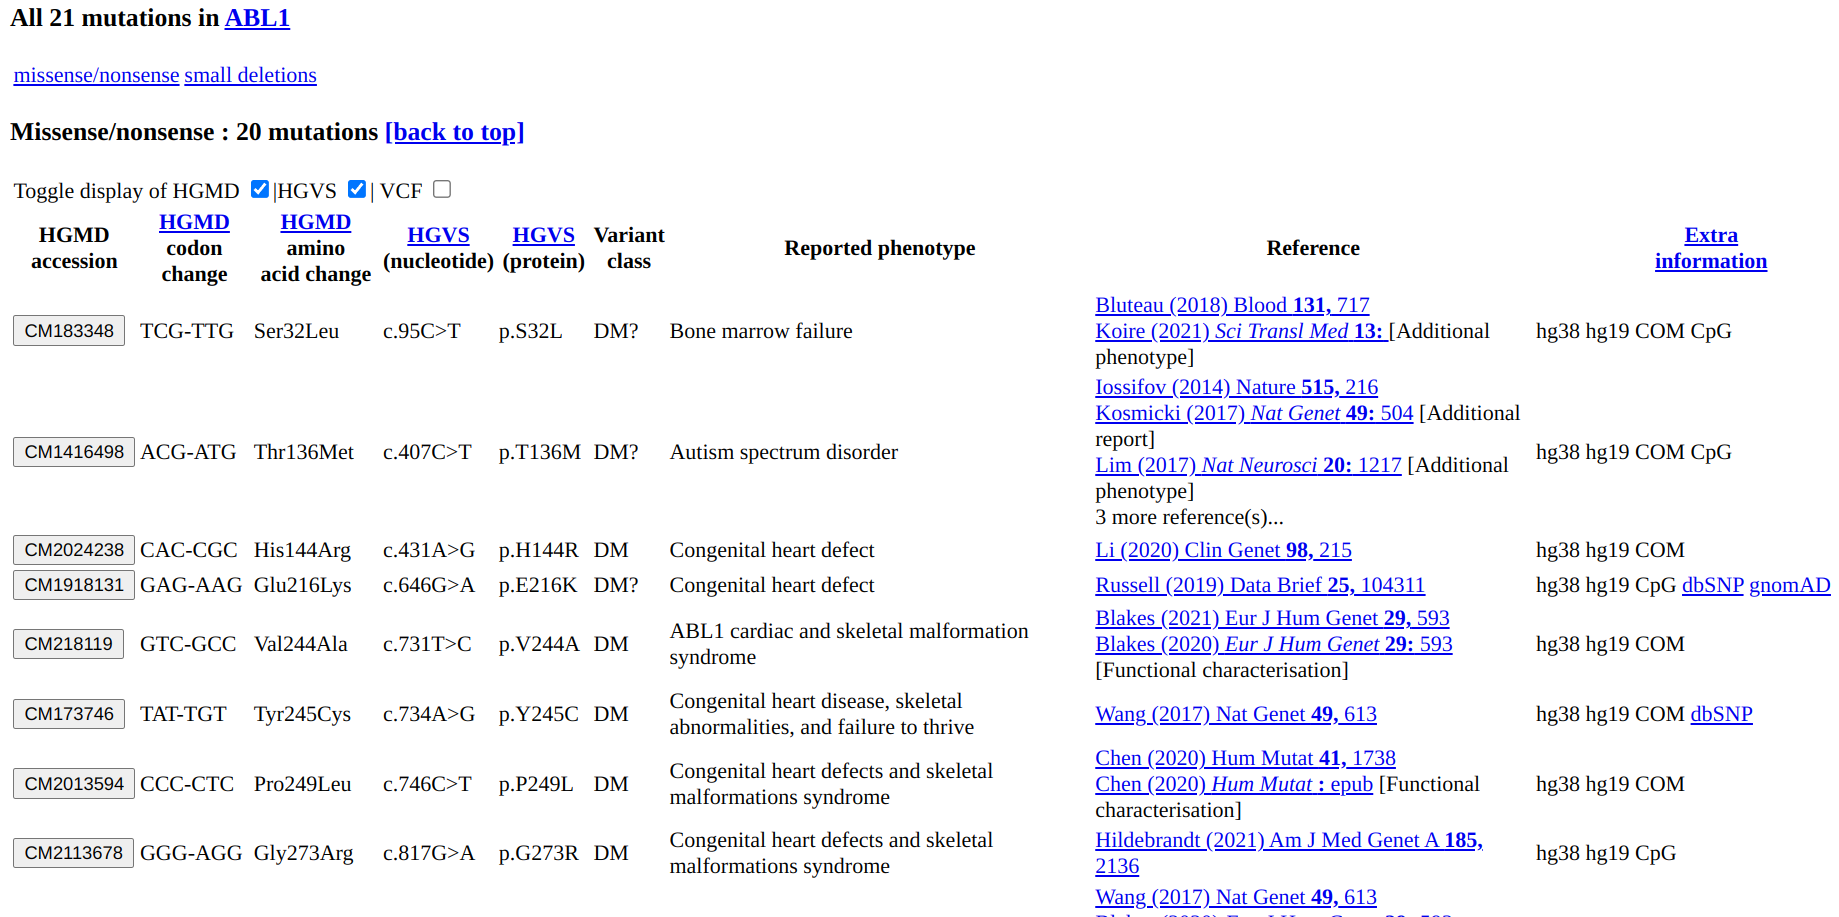
\includegraphics[width=1.1\linewidth]{Hinh_ve/HGMD_ABL1.png}
\caption{Kết quả trả về khi tìm kiếm từ khóa ABL1 trên HGMD pro}
\label{fig:HGMDABL1}
\end{figure}

\begin{figure}
\centering
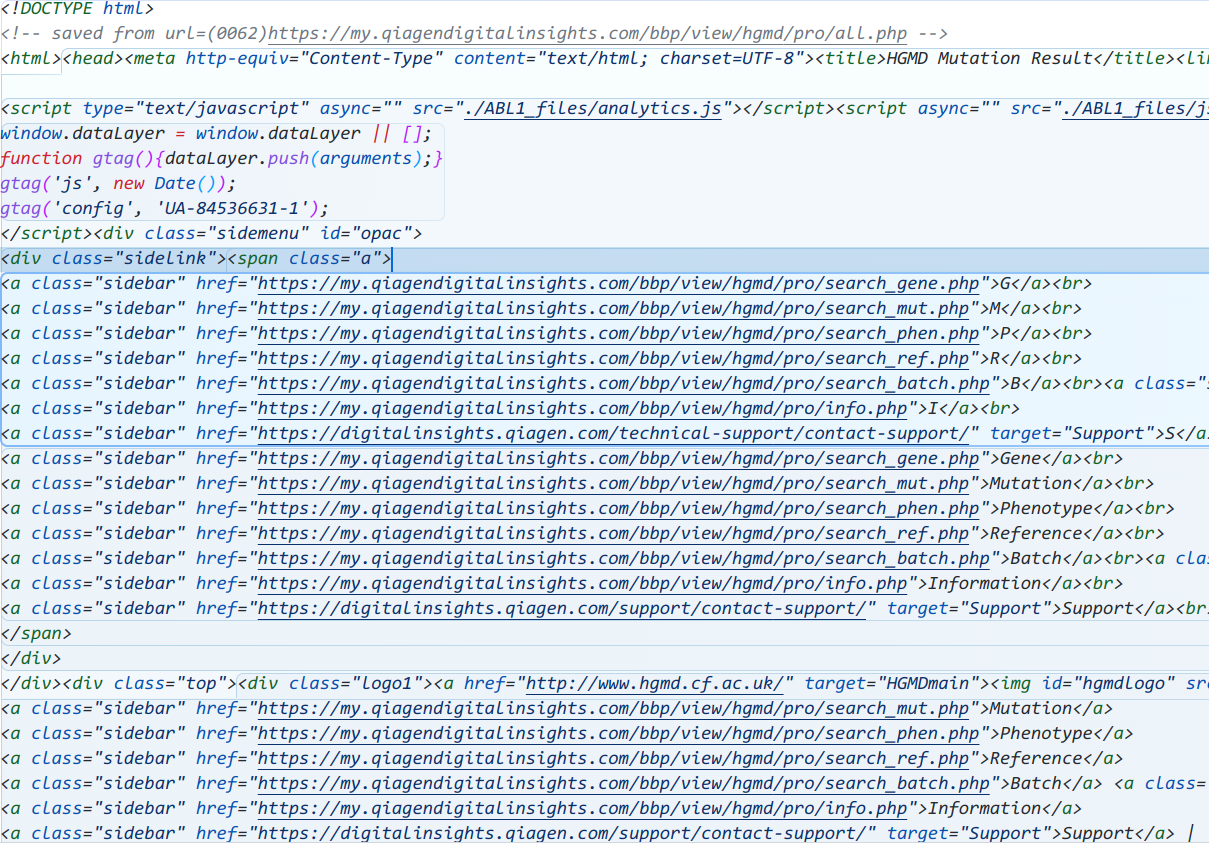
\includegraphics[width=1\linewidth]{Hinh_ve/html_hgmd_pro.png}
\caption{Nội dung của file html lấy được từ HGMD}
\label{fig:htmlHgmd}
\end{figure}

Bước 4: Lớp (âm tính) negative gồm 100299 bài báo được lấy ngẫu nhiên từ \href{https://ftp.ncbi.nlm.nih.gov/pub/pmc/}{PubMed Central}. Toàn bộ 225149 bài báo là không trùng nhau. Không có bài báo nào xuất hiện nhiều hơn một lần, và không có bài báo nào vừa thuộc positive, vừa thuộc negative. Thống kê về số lượng data ở mỗi lớp được thể hiện ở hình \ref{fig:3cls}. Nhìn vào biểu đồ phân bố dữ liệu có thể thấy việc mất cân bằng dữ liệu là nhỏ. Nên bỏ qua vấn đề này.

% classify tiêu đề và tóm tắt
\section{Phân loại tiêu đề và tóm tắt bài báo}

\subsection{Xây dựng mô hình phân loại văn bản}
\subsubsection{Tiền xử lý dữ liệu}
Dữ liệu thu thập phía trên được tiền xử lý trước khi tiến hành phân loại. Các kỹ thuật tiền xử lý văn bản được áp dụng gồm có 5 bước như hình \ref{fig:pretext}
\begin{figure}
\centering
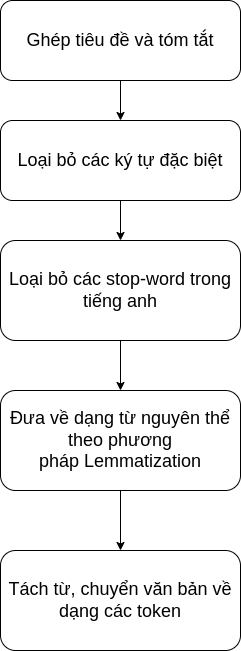
\includegraphics[width=0.5\linewidth]{Hinh_ve/preprocessingtext.png}
\caption{Các bước tiền xử lý văn bản trước khi huấn luyện mô hình}
\label{fig:pretext}
\end{figure}

Vì có một số lượng đáng kể các bài báo được lưu trữ tại Pubmed là không có phần tóm tắt, vì thế em đã quyết định nối 2 văn bản này thành 1 văn bản duy nhất, tránh được việc có những điểm dữ liệu bị trống. Hàm để xử lý ghép tiêu đề và tóm tắt được sử dụng như phía dưới.
\begin{lstlisting}
def concat_title_abstract(title,abstract) -> str:
    text = title + abstract
    return text
\end{lstlisting}

Các tác giả bài báo thường có xu hướng không sử dụng công thức toán học hay các ký tự đặc biệt ở phần tiêu đề và tóm tắt của bài báo. Vì thế, nếu có ký tự đặc biệt ở đây, khả năng cao là nhiễu và chúng cũng không mang nhiều ý nghĩa. Vì thế các ký tự đặc biệt cần được loại bỏ để tăng hiệu năng cho mô hình phân loại. 
\begin{lstlisting}
def remove_daucau(text):
    patt= r"""[!"#$%&'()*+,-./:;<=>?@[\]^_`{|}~]"""
    text = re.sub(patt, '', text)
    return text
\end{lstlisting}

Các stop-word trong tiếng anh ví dụ như "a", "an", "the", ... có tần suất xuất hiện rất nhiều. Tuy nhiên, chúng lại không mang quá nhiều thông tin đáng kể đến nội dung của văn bản y khoa như tiêu đề và tóm tắt. Vì thế ta sẽ tiến hành loại bỏ những từ này ra khỏi văn bản.
\begin{lstlisting}
import nltk
from nltk.corpus import stopwords
swords = set(stopwords.words('english'))
def remove_stopword(text):
    otokens = word_tokenize(text)
    ntokens=[w for w in otokens if w not in swords]
    newtext = ' '.join(ntokens)
    return newtext

\end{lstlisting}
Vì các văn bản khoa học đều có nội dung khách quan, vì thế các dạng khác nhau của từ chỉ mang thêm các thông tin chủ quan như từ ở dạng số nhiều/ số ít, tính từ/ động từ / danh từ / trạng từ. Nếu đưa tất cả về dạng nguyên thế, sẽ làm giảm đang kể kích thước của từ điển. Trong khi hiệu năng phân loại của mô hình không thay đổi đáng kể. Thêm vào đó, việc giảm kích thước từ điển sẽ giúp cải thiện khá nhiều về tốc độ phân loại văn bản. Vì vậy việc chuyển về dạng nguyên thể của từ là một việc làm có ý nghĩa và là một việc quan trọng cần thực hiện.
\begin{lstlisting}
import nltk
nltk.download('punkt')
from nltk.stem import WordNetLemmatizer
lemma = WordNetLemmatizer()
def convert_word(text:str) -> str:
    otokens = word_tokenize(text)
    ntokens = []
    for token in otokens:
        w = lemma.lemmatize(token,pos ="a")
        ntokens.append(w)
    return ' '.join(ntokens)
\end{lstlisting}

Tách từ cũng là một công việc quan trọng. Tuy nhiên, không giống như tiếng việt, mỗi 1 tiếng trong anh đều là một từ trong tiếng anh. Vì thế, việc tách từ và tokenized hóa trong tiếng anh là một việc tương đối dễ dàng với sự hỗ trợ của thư viện ``nltk``
\begin{lstlisting}
from nltk.tokenize import sent_tokenize
def convert_work2token(text) -> str:
    return sent_tokenize(text)
\end{lstlisting}


\subsubsection{Xây dựng mô hình phân loại}
Sau quá trình tiền xử lý, em đã chuyển văn bản về dạng count vector, rồi chuyển tiếp về dạng tf-idf \cite{salton1975vector} , count vector là kỹ thuật xây dựng từ điển chứa tất cả các từ trong bộ dữ liệu. 
Ví dụ từ điển có những từ sau : ['tôi', 'thích', 'đá', 
'bóng']. Như vậy với một câu "tôi thích bóng". Khi cần chuyển về thành count vector sẽ có giá trị là [1, 1, 0, 1]. Có thể thấy rằng câu "tôi thích bóng" có 3 từ xuất hiện trong từ điển. mà 3 từ này lại có số thứ tự 1, 2, và 4, nên vector đại diện cho câu "tôi thích bóng" sẽ là [1, 1, 0, 1]. Khi đó mỗi văn bản là một vector có độ dài bằng kích thước của từ điển. Khi đó, ứng mới mỗi từ xuất hiện trong câu, ta có tại vị trí của từ đó, giá trị của vector biểu diễn cho văn bản sẽ cộng thêm 1. Phương pháp count vector này có nhược điểm là không xác định được tầm quan trọng của một từ trong toàn bộ văn bản. vì đôi khi một từ hiếm gặp nhưng lại quan trong đối với văn bản đó. Chính vì vậy, phương pháp tf-idf \cite{salton1975vector} giải quyết được điều này bằng cách xác định tần suất xuất hiện của từ đó trong từ điển. Vì thế, ta áp dụng phương pháp tf-idf để thu được vector đặc trưng đại diện cho một bài báo khoa học. Đoạn chương trình dùng để chuyển văn bản về dạng count vector rồi chuyển qua term vector được thực hiện như sau:

\begin{lstlisting}
from sklearn.feature_extraction.text import \
    CountVectorizer, TfidfTransformer
    
count_vec = CountVectorizer()
tfidf_trans = TfidfTransformer()
def convert2TFIDF(df:pd.DataFrame):
    X_counts=count_vec.fit_transform(df["text"].str)
    X_tfidf = tfidf_trans.fit_transform(X_counts)
    return X_tfidf
\end{lstlisting}

Sau đó, em sử dụng phương pháp K-fold với K = 5, 
phương pháp này sẽ chia toàn bộ bộ dữ liệu ra thành 5 phần bằng nhau. Với mỗi lần huấn luyện, ta sẽ chọn ra 4 phần dữ liệu để huấn luyện và 1 phần dũ liệu còn lại để tiến hành kiểm tra. Lặp lại với 5 lần thương tự như lần huấn luyện đầu tiên, ta chọn ra mô hình có các chỉ số đánh giá là tốt nhất trên bộ dữ liệu huấn luyện. Như vậy, tỉ lệ dữ liệu huấn luyện trên dữ liệu kiểm tra là 0.8 / 0.2. Sau đó ta tiến hành huấn luyện một loạt các thuật toán học máy bao gồm k-nearest neighbors với K=4, Bernoulli Naive bayes, Multinomial Naive bayes, Complement Naive bayes, LogisticRegression, và SVM tuyến tính để chọn ra để chọn ra mô hình tối ưu nhất, có chỉ số recall là cao nhất. 
\textbf{Đoạn chương trình huấn luyện và đánh giá mô hình k-nearest neighbors với K=4}
\begin{lstlisting}
from sklearn.neighbors import KNeighborsClassifier

clf=KNeighborsClassifier(n_neighbors=4).fit(Xtrain,ytrain)
y_pred_proba = clf.predict_proba(Xtest)[::,1]
fpr, tpr, _ = metrics.roc_curve(ytest, y_pred_proba)
y_pred_proba = clf.predict_proba(Xtest)[::,1]
fpr, tpr, _ = metrics.roc_curve(ytest,y_pred_proba)
auc = metrics.roc_auc_score(ytest, y_pred_proba)

plt.plot(fpr,tpr,label="AUC="+str(auc))
plt.ylabel('True Positive Rate')
plt.xlabel('False Positive Rate')
plt.legend(loc=4)
plt.show()
\end{lstlisting}
\textbf{Đoạn chương trình huấn luyện và đánh giá mô hình Bernoulli Naive bayes}
\begin{lstlisting}
from sklearn.naive_bayes import BernoulliNB

clf = BernoulliNB().fit(X_train, y_train)
y_pred_proba = clf.predict_proba(X_test)[::,1]
fpr, tpr, _ = metrics.roc_curve(y_test,  y_pred_proba)
y_pred_proba = clf.predict_proba(X_test)[::,1]
fpr, tpr, _ = metrics.roc_curve(y_test,  y_pred_proba)
auc = metrics.roc_auc_score(y_test, y_pred_proba)

plt.plot(fpr,tpr,label="AUC="+str(auc))
plt.ylabel('True Positive Rate')
plt.xlabel('False Positive Rate')
plt.legend(loc=4)
plt.show()
\end{lstlisting}

\textbf{Đoạn chương trình huấn luyện và đánh giá mô hình Logistic Regression}
\begin{lstlisting}
from sklearn.linear_model import LogisticRegression

clf = LogisticRegression().fit(X_train, y_train)
y_pred_proba = clf.predict_proba(X_test)[::,1]
fpr, tpr, _ = metrics.roc_curve(y_test,  y_pred_proba)
y_pred_proba = clf.predict_proba(X_test)[::,1]
fpr, tpr, _ = metrics.roc_curve(y_test,  y_pred_proba)
auc = metrics.roc_auc_score(y_test, y_pred_proba)

plt.plot(fpr,tpr,label="AUC="+str(auc))
plt.ylabel('True Positive Rate')
plt.xlabel('False Positive Rate')
plt.legend(loc=4)
plt.show()
\end{lstlisting}
\textbf{Đoạn chương trình huấn luyện và đánh giá mô hình Multinomial Naive bayes}
\begin{lstlisting}
from sklearn.naive_bayes import MultinomialNB

clf = MultinomialNB().fit(X_train, y_train)
y_pred_proba = clf.predict_proba(X_test)[::,1]
fpr, tpr, _ = metrics.roc_curve(y_test,  y_pred_proba)
y_pred_proba = clf.predict_proba(X_test)[::,1]
fpr, tpr, _ = metrics.roc_curve(y_test,  y_pred_proba)
auc = metrics.roc_auc_score(y_test, y_pred_proba)

plt.plot(fpr,tpr,label="AUC="+str(auc))
plt.ylabel('True Positive Rate')
plt.xlabel('False Positive Rate')
plt.legend(loc=4)
plt.show()
\end{lstlisting}

\textbf{Đoạn chương trình huấn luyện và đánh giá mô hình Complement Naive Bayes}
\begin{lstlisting}
from sklearn.naive_bayes import ComplementNB

clf = ComplementNB().fit(X_train, y_train)
y_pred_proba = clf.predict_proba(X_test)[::,1]
fpr, tpr, _ = metrics.roc_curve(y_test,  y_pred_proba)
y_pred_proba = clf.predict_proba(X_test)[::,1]
fpr, tpr, _ = metrics.roc_curve(y_test,  y_pred_proba)
auc = metrics.roc_auc_score(y_test, y_pred_proba)

plt.plot(fpr,tpr,label="AUC="+str(auc))
plt.ylabel('True Positive Rate')
plt.xlabel('False Positive Rate')
plt.legend(loc=4)
plt.show()
\end{lstlisting}
\textbf{Đoạn chương trình huấn luyện và đánh giá mô hình Suport Vector machine với hạt nhân tuyến tính}
\begin{lstlisting}
from sklearn.svm import LinearSVC

clf = LinearSVC().fit(X_train, y_train)
y_pred_proba = clf.predict_proba(X_test)[::,1]
fpr, tpr, _ = metrics.roc_curve(y_test,  y_pred_proba)
y_pred_proba = clf.predict_proba(X_test)[::,1]
fpr, tpr, _ = metrics.roc_curve(y_test,  y_pred_proba)
auc = metrics.roc_auc_score(y_test, y_pred_proba)

plt.plot(fpr,tpr,label="AUC="+str(auc))
plt.ylabel('True Positive Rate')
plt.xlabel('False Positive Rate')
plt.legend(loc=4)
plt.show()
\end{lstlisting}

Toàn bộ quá trình này gồm trích chọn đặc trưng và huấn luyện mô hình em đã sử dụng thư viện scikit learn để thực hiện. Để đánh giá mô hình nào là phù hợp, với mong muốn lấy được nhiều nhất bài báo khoa học thuộc về lớp positive (bài báo liên quan đến bệnh ung thư), thuật toán nào có chỉ số recall cao nhất sẽ được chọn. Tuy nhiên, để đánh giá xem mô hình phân loại văn bản y khoa có tốt không hay, ta vẫn cần đánh giá mô hình thông qua các chỉ số khác như F1 score, AUC, đường cong ROC.

\section{Tải xuống bài báo và chuyển sang dạng văn bản (txt)}
\begin{figure}
\centering
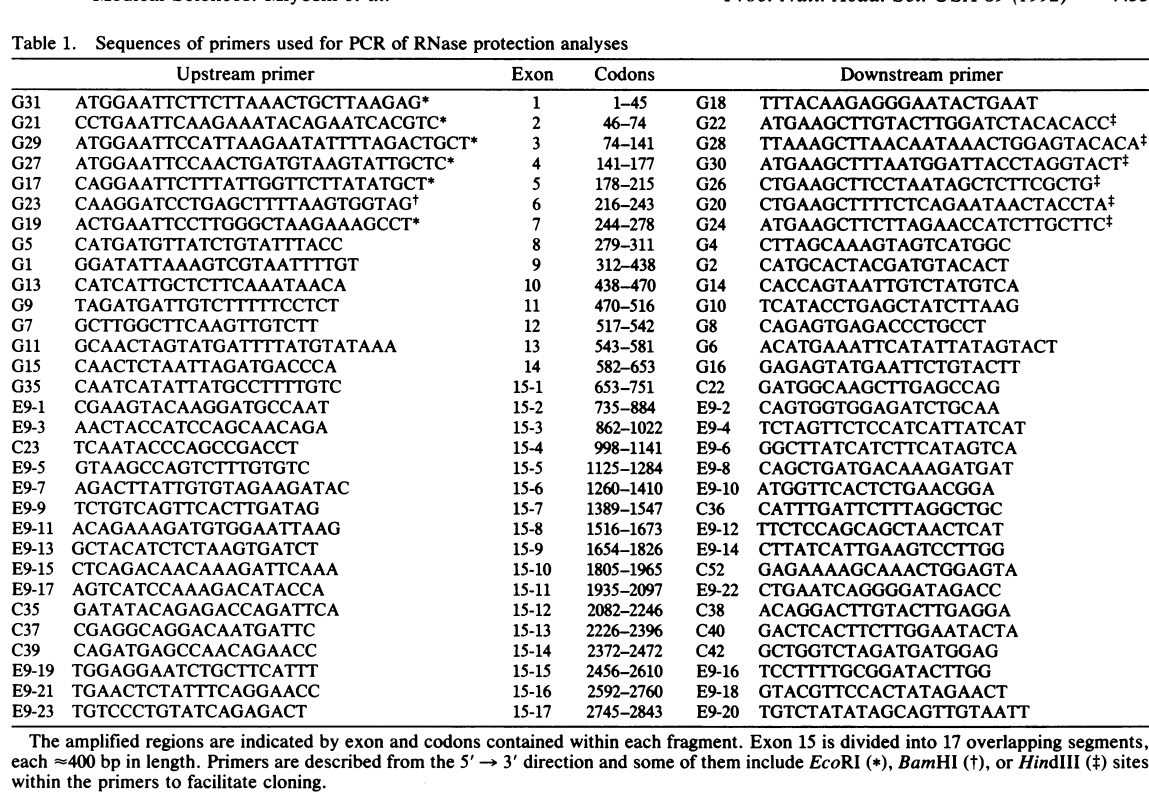
\includegraphics[width=1.0\linewidth]{Hinh_ve/PDFraw.png}
\caption{Nội dung ban đầu của bài báo khoa học ở dạng PDF, Bảng này được lấy từ bài báo có tiêu đề ``Germ-line mutations of the APC gene in 53 familial adenomatous polyposis patients``, nội dung đầy đủ của bài báo có thể xem tại đường dẫn ``https://www.ncbi.nlm.nih.gov/pmc/articles/PMC49100/``.}
\label{fig:PDFraw1316610}
\end{figure}

\begin{figure}
\centering
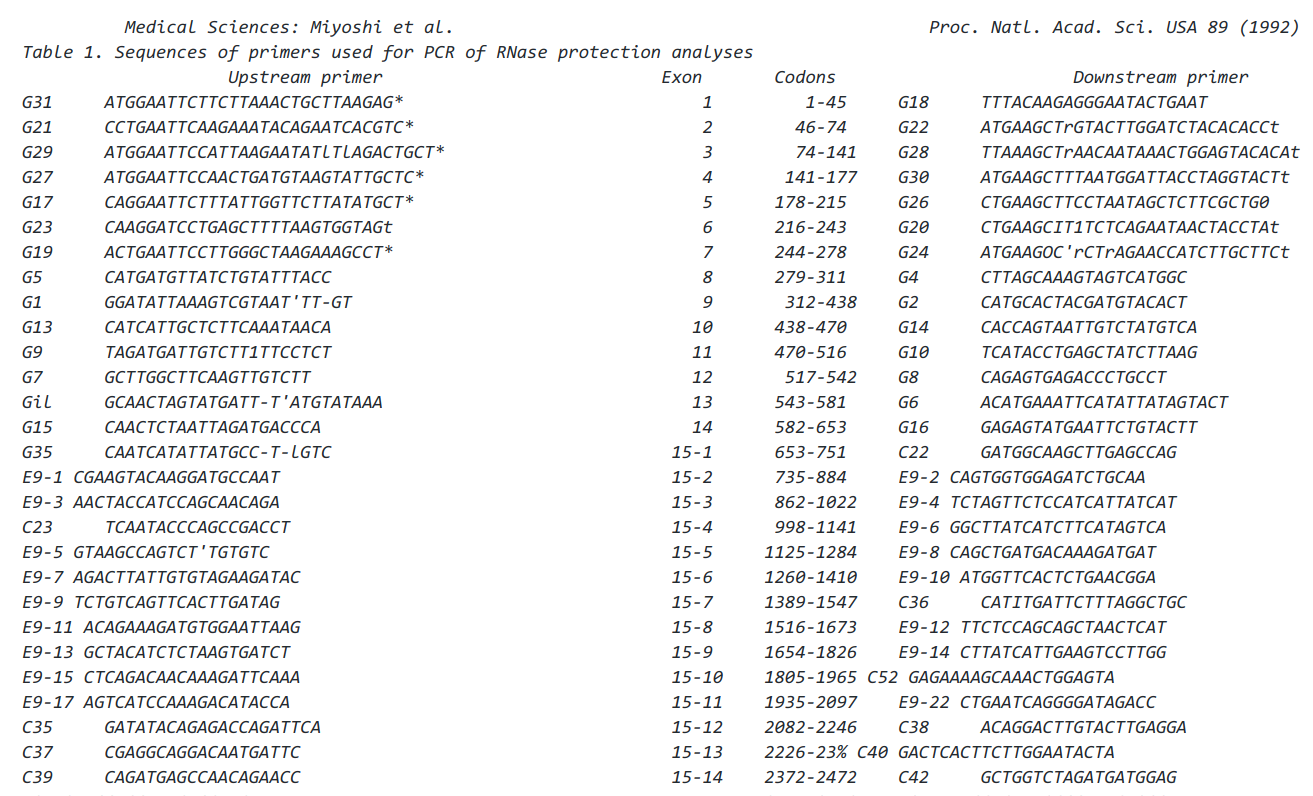
\includegraphics[width=1.\linewidth]{Hinh_ve/popller.png}
\caption{Chuyển đổi bài báo khoa học từ định dạng ".pdf" sang định dạng ".txt" sử dụng thư viện python poppler\cite{poppler}, có thể thấy rằng, thư viện python-poppler giữ nguyên được cấu trúc của bài báo khi chuyển đổi từ định dạng pdf.}
\label{fig:poppler}
\end{figure}

\begin{figure}
\centering
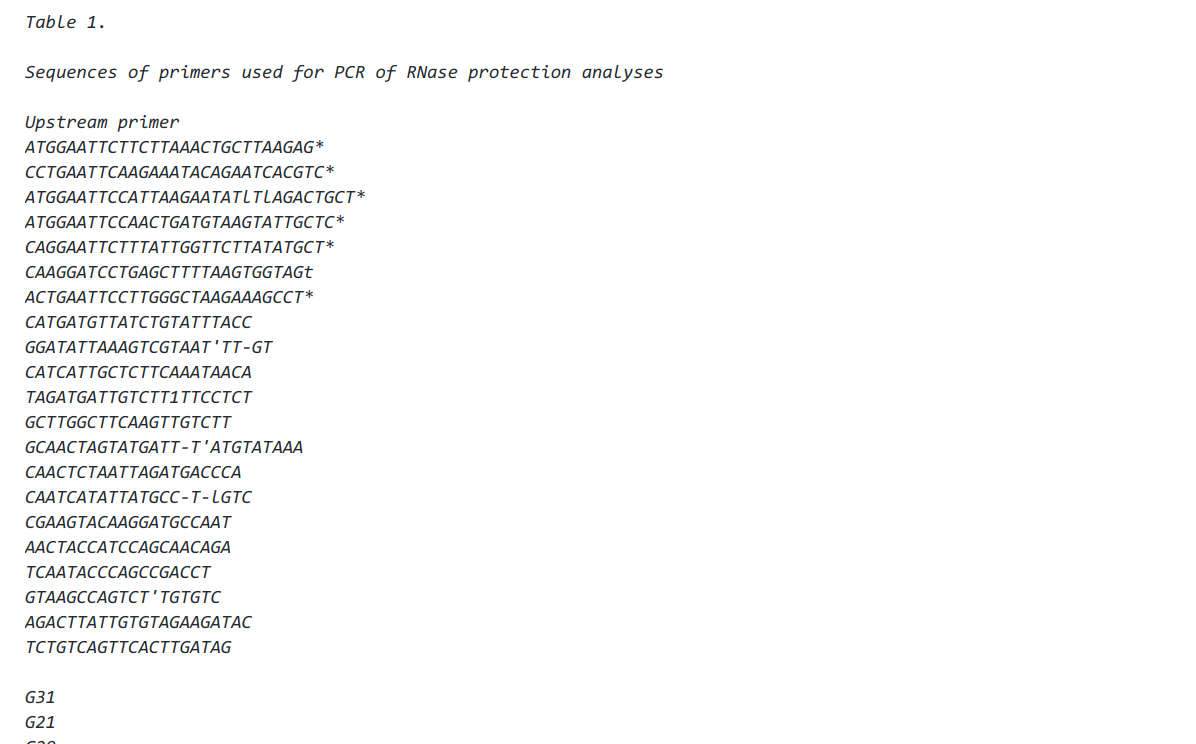
\includegraphics[width=1.5\linewidth]{Hinh_ve/notPopller.png}
\caption{Chuyển đổi bài báo khoa học từ định dạng ".pdf" sang định dạng ".txt" sử dụng các thư viện PDFminer. Có thể thấy rằng, định dạng bảng 1bên trong bài báo PDF đã bị phá vỡ hoàn toàn}
\label{fig:pdfother}
\end{figure}

\begin{figure}
\centering
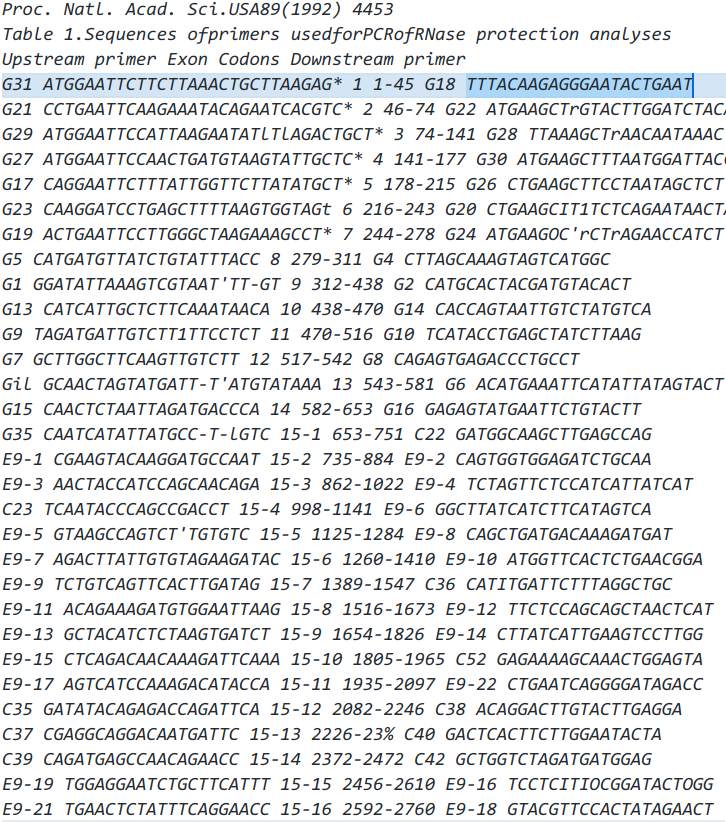
\includegraphics[width=1.0\linewidth]{Hinh_ve/notPopller_pyPDF2.png}
\caption{Chuyển đổi bài báo khoa học từ định dạng ".pdf" sang định dạng ".txt" sử dụng các thư viện PyPDF2, có thể thấy rằng, các ô trong bảng nằm trên cùng một dòng đã bị nối vào nhau. Việc này cũng gây ra sai lệch thông tin.}
\label{fig:Pypdf2}
\end{figure}

Kết thúc bước 2, nếu bài báo được xác định là có liên quan đến ung thư sẽ được tải xuống toàn bộ bài báo ở dạng pdf. Sau đó, em sử dụng thư viện python-poppler để chuyển bài báo từ dạng pdf sang dạng file txt. Thư viện python-poppler chuyển đổi bài báo từ dạng \textbf{pdf} \ref{fig:PDFraw1316610} sang dạng txt có thể giữ được nguyên cấu trúc của bài báo \textbf{hình} \ref{fig:poppler}. Trong khi các thư viện khác như PDFminer, \textbf{hình} \ref{fig:pdfother}, hay thư viện PyPDF2 \textbf{hình} \ref{fig:Pypdf2} , định dạng text thu được sau khi convert đã khiến các ô trong bảng bị dính vào nhau. Trong trường hợp biến thể cần tìm được bài báo trình bày trong bảng, cấu trúc đoạn gene phía trong đã không tuân theo tiêu chuẩn danh pháp HGSV. Điều này là quan trọng vì các biến thể gây ung thư có đề được mô tả trong bảng biểu, trong chú thích của hình ảnh. Ngoài ra, các biến thể còn chứa các ký tự đặc biệt. Vì vậy việc giữ đúng định dạng giống bài báo ở dạng pdf ban đầu là rất quan trọng. Nó hạn chế việc bỏ sót không tìm thấy các biến thể do nội dung đã bị biến dạng khi chuyển đổi qua lại giữa các định dạng file.

\section{Tìm kiếm các biến thể được mô tả trong bài báo}
\subsection{Tiêu chuẩn danh pháp HGVS}

\begin{figure}
\centering
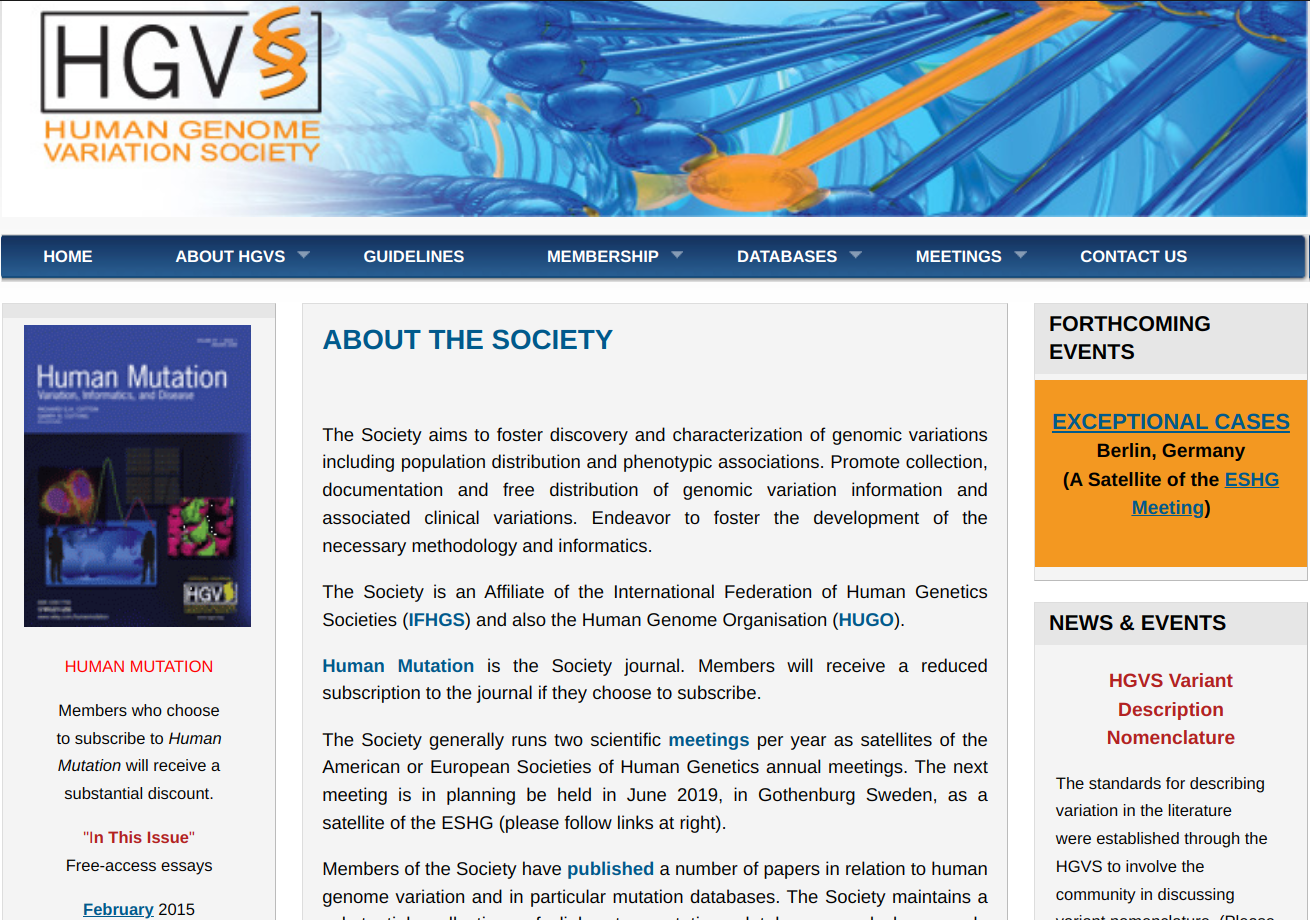
\includegraphics[width=1.0\linewidth]{Hinh_ve/HGVShomepage.png}
\caption{Trang chủ của tổ chức Human Genome Variation Society - HGVS}
\label{fig:HGVSHomepage}
\end{figure}
Những thay đổi trong các chuỗi DNA, RNA, hay protein được gọi chung là biến thể (variants), hoặc đột biến (mutations), hoặc đa hình (polymorphisms). Những thay đổi này được mô tả bằng một ngôn ngữ đặc biệt có tên là "Tiêu chuẩn danh pháp HGVS" (HGVS nomenclature standard) \cite{HGVS} . Tiêu chuẩn này được đưa ra bởi hiệp hội đột biến gene người (human genome variation society - HGVS). Tiêu chuẩn này được sử dụng chính thức trên toàn thế giới, đặc biệt là trong lĩnh vực chăm sóc sức khỏe con người và chẩn đoán lâm sàng. HGVS đưa ra cú pháp để mô tả các biến thể xảy ra trên các đoạn mã di truyền như DNA, RNA, protein, \ldots Các tiêu chuẩn để mô tả biến thể / đột biến được thiết lập thông qua HGVS để cộng đồng có thể tham gia thảo luận về danh pháp biến thể. Hiện nay, lĩnh vực danh pháp đã đạt đến mức bắt buộc phải thiết lập các tiêu chuẩn quốc tế được công nhận rộng rãi, điều này nhằm mục đích tạo điều kiện thuận lợi cho công việc nghiên cứu và chẩn đoán lâm sàng về biến dị di truyền trong tương lai.

\subsubsection{Một số loại đột biến phổ biến xảy ra trên DNA}
Có nhiều loại đột biến có thể xảy ra trên DNA. Trong đó các loại đột biến xuất hiện phổ biến như: 

Đột biến thay thế (\textit{Substitution Variant}) khi so với trình tự tham chiếu, một nucleotide được thay thế bằng một nucleotide khác. Để mô tả loại đột biến này, ta sử dụng cú pháp \begin{center}“prefix”“PositionSubstituted”“ReferenceNucleotide””>””NewNucleotide”\end{center}
 Trong đó “prefix” là trình tự tham chiếu được sử dụng, “PositionSubstituted” là vị trí xảy ra đột biến thay thế, “ReferenceNucleotide” là nucleotide ở vị trí tham chiếu, ”>” ký hiệu để biểu diễn chuỗi ký tự này mô tả đây là loại đột biến thay thế, ”NewNucleotide” là nucleotide thay thế. Ví dụ "g.123A>G", g là trình tự tham chiếu được sử dụng được tham chiếu đến, 123 là vị trí xảy ra đột biến, A, là nucleotide ở vị trí tham chiếu, ">" mô tả đây là đột biến thay thế, G là nucleotide mới.

 Đột biến mất đoạn (\textit{Deletion Variant}), đây là 1 loại đột biến nguy hiểm nhất, khi so sánh với trình tự tham chiếu, một hoặc nhiều nucleotide không có mặt (bị xóa). Để biểu diễn loại đột biến này, ta sử dụng cú pháp: 
 \begin{center}“prefix”“Position(s)Deleted”“del”\end{center}
Trong đó, “Prefix” là trình tự tham chiếu được sử dụng, “Position (s) Deleted” = vị trí nucleotide bị xóa (nếu chỉ một nucleotide bị xóa) hoặc phạm vi nucleotide bị xóa(nếu nhiều nucleotide bị xóa). “Del” biểu diễn rằng loại đột biến này là đột biến mất đoạn (Deletion Variant). Ví dụ g.123-127del , trong đó g là trình tự tham chiếu được sử dụng, 123-127 tức vị trí xảy ra đột biến mất đoạn là từ vị trí 123 đến 127, del nghĩa là đây là đột biến mất đoạn.

 Đột biến lặp đoạn (\textit{Duplication Variant}), so với trình tự tham chiếu, bản sao của một hoặc nhiều nucleotit được chèn trực tiếp vào đoạn DNA đó khi so với bản sao gốc của DNA đó. Để biểu diễn loại đột biến này, ta sử dụng cú pháp: 
 \begin{center}“prefix”“position(s)-duplicated”“dup”\end{center}
Ví dụ  g.123-345dup. Trong đó “Prefix” = trình tự tham chiếu được sử dụng = g. “Position (s) -duplicated” = vị trí nucleotide hoặc phạm vi nucleotide được nhân đôi = 123-345. “dup” = loại đột biến là đột biến lặp đoạn (Duplication Variant).

 Đột biến thêm đoạn (\textit{Insertion Variant}), là một loại đột biến trong đó, khi so sánh với trình tự tham chiếu, một hoặc nhiều nucleotit được chèn vào và nơi phần chèn không phải là bản sao của trình tự cũ. Đột biến này không phải là đột biến lặp đoạn. Để mô tả loại đột biến này, ta sử dụng cú pháp 
 \begin{center}“prefix”“positions-flanking”“ins”“inserted-sequence”\end{center} 
 Ví dụ g.123-124insAGC. Trong đó, “Prefix” = trình tự tham chiếu được sử dụng = g, “Position-flanking” = vị trí của hai nucleotide bên cạnh nucleotide bị chèn vào = 123-124, “ins” = loại đột biến là đột biến thêm đoạn (Insertion Variant) = ins, “inserted-sequence” = trình tự đã chèn = AGC.

 Đột biến xóa chèn (\textit{Deletion-insertion Variant}), đây là loại đột biến trong đó khi so sánh với trình tự tham chiếu, một hoặc nhiều nucleotit được thay thế bằng một hoặc nhiều nucleotit khác và không phải là đột biến thay thế, đột biến đảo ngược hoặc đột biến chuyển đổi. đột biến này là mất đoạn hay thêm đoạn phụ thuộc vào từng trường hợp khi ta so sanh với trình tự tham chiếu. Để biểu diễn đột biến này, ta sử dụng cú pháp: 
 \begin{center}“prefix”“position(s)-deleted”“delins”“inserted-sequence”\end{center}
 Ví dụ: g.123-127delinsAG. Trong đó, “Prefix” = trình tự tham chiếu được sử dụng = g. “Position (s) -deleted” = vị trí nucleotide hoặc phạm vi nucleotide bị xóa = 123-127, “Delins” = loại đột biến là xóa-chèn = delins, “Insert-sequence” = mô tả trình tự nucleotide xảy ra dột biến = AG.

\subsubsection{Một số loại đột biến phổ biến xảy ra trên protein}
 Có nhiều loại đột biến có thể xảy ra trên Protein. Trong đó các loại đột biến xuất hiện phổ biến như: 
 
Đột biến thay thế (\textit{Substitution Variant}) là một loại đột biến trong đó khi so sánh với trình tự tham chiếu, một axit amin được thay thế bằng một axit amin khác. Để biểu diễn đột biến này, ta sử dụng cú pháp: 
\begin{center}“prefix”“amino-acid”“position”“new-amino-acid”\end{center}
Ví dụ: p.(Arg54Ser). Trong đó, “Prefix” = trình tự tham chiếu được sử dụng = p. “Amino-acid” = amin được sử dụng để tham chiếu đến = Arg. “Position” = vị trí axit amin được thay thế = 54. “New-amino-acid” = axit amin mới = Ser. 

Đột biến mất đoạn (\textit{Deletion Variant}) sự thay đổi trình tự giữa codon bắt đầu dịch mã (bắt đầu) và kết thúc (dừng) trong đó, so với trình tự tham chiếu, một hoặc nhiều axit amin không có mặt (bị xóa). Để biểu diễn loại đột biến này, ta sử dụng cú pháp: 
\begin{center}“prefix”“amino-acid(s)+position(s)-deleted”“del”\end{center}\
Ví dụ: p.(Cys76-Glu79del). Trong đó: “Prefix” = trình tự tham chiếu được sử dụng = p. “Amino-acid (s) + position (s)-deleted” = axit amin có vị trí hoặc phạm vi (axit amin đầu tiên có vị trí đến axit amin cuối cùng có vị trí) bị xóa = Cys76-Glu79. “Del” = loại đột biến là đột biến mất đoạn = del.

Đột biến thêm đoạn (\textit{Insertion Variant}) là một loại đột biến làm thay đổi vị trí giữa codon bắt đầu dịch mã và và codon kết thúc dịch mã. Trong đó, khi so sách với trình tự tham chiếu, một hoặc nhiều axit amin được chèn vào, đây không phải là đột biến chuyển đoạn (frame shift) và axit amin được chèn vào không phải là bản sao của axit amin đã xuất hiện trong chuỗi, phân biệt với đột biến mất đoạn. Để biểu diễn loại đột biến này, ta sử dụng cú pháp:
\begin{center}“prefix”“amino-acids+positions-flanking”“ins”“inserted-sequence”\end{center}
Ví dụ:  p.(Lys23-Leu24insArgSerGln) Trong đó: “Prefix” = trình tự tham chiếu được sử dụng = p. “Amino-acids + position-flanking” = axit amin có vị trí chèn bên cạnh = Lys23-Leu24. “Ins” = loại đột biến là đột biến thêm đoạn (\textit{Insertion Variant}) = ins. “Insert-sequence” = chuỗi amino axit chèn vào = ArgSerGln.

Đột biến chuyển đoạn (\textit{Frame shift Variant}) là một loại đột biến làm trình tự giữa codon bắt đầu phiên mã và codon kết thúc phiên mã. trong đó, so với trình tự tham chiếu, dịch chuyển sang một chuỗi khác. Để biểu diễn loại đột biến này, ta sử dụng cú pháp:
\begin{center}  “prefix”“amino-acid”position”new-amino-acid”“fs”“Ter”“position-termination-site”\end{center}
Ví dụ: p.(Arg123LysfsTer34). Trong đó: “Prefix” = trình tự tham chiếu được sử dụng = p. “Amino-acid” = axit amin đầu tiên bị thay đổi = Arg. “Position” = vị trí xảy ra đột biến = 123. “New-amino-acid” = axit amin mới đã thay thế axit amin cũ = Lys. “fs” = loại đột biến này là đột biến chuyển đoạn (\textit{Frame shift Variant}) = fs. “Ter” = codon kết thúc = Ter. “Position-termina-site” = vị trí kết thúc mới = 34.


\subsection{Xây dựng biểu thức chính quy tìm kiếm biến thể}
\begin{table}[]
\centering
\caption{Số lượng biểu thức chính quy ứng với mỗi loại đột biến được sử dụng để tìm kiếm các biến thể được mô tả trong bài báo khoa học.}
\label{tab:regextable}
\begin{tabular}{@{}lcc@{}}
\toprule
\textbf{Loại đột biến}         & \textbf{DNA} & \textbf{Protein} \\ \midrule
mất đoạn (deletion)            & 11           & 6                \\
\cmidrule đảo đoạn (frameshift) & 4            & 0                \\
lặp đoạn (duplicate )          & 3            & 0                \\
thêm đoạn (insertion)          & 3            & 4                \\
thay thế (subsituation)        & 4            & 5                \\
cắt nối (splicing)             & 2            & 0                \\
delins                         & 4            & 0                \\
ivssub                         & 1            & 0                \\ \bottomrule
\end{tabular}
\end{table}

Vì các biến thể được nhắc đến trong các bài báo khoa học tuân theo "tiêu chuẩn danh pháp HGVS" \cite{HGVS} . Vì thế ta có thể sử dụng biểu thức chính quy để tìm kiếm biến thể. Em đã sử dụng 47 biểu thức chính quy để tìm kiếm các biến thể. Biểu thức chính quy này mô tả các loại đột biến xảy ra trên DNA hoặc Protein, các loại đột biến có thể tìm thấy gồm thay thế (substitution), thêm đoạn (insertion), mất đoạn (deletion), đảo đoạn (frameshift), lặp đoạn (duplication), cắt nối (splicing) .Biến thể hợp lệ là một chuỗi ký tự có khuôn mẫu khớp với ít nhất 1 trong 47 biểu thức chính quy. Chi tiết số lượng ứng với từng loại đột biến được mô tả trong \textbf{bảng} \ref{tab:regextable}. Do các biểu thức chính quy chứa rất nhiều ký tự đặc biệt , nên danh sách cụ thể biểu thức chính quy em đã lưu tại đường dẫn  \begin{verbatim}https://tinyurl.com/3c2zrx86\end{verbatim} Toàn bộ source code em cũng đã lưu tại đây.

\begin{figure}
\centering
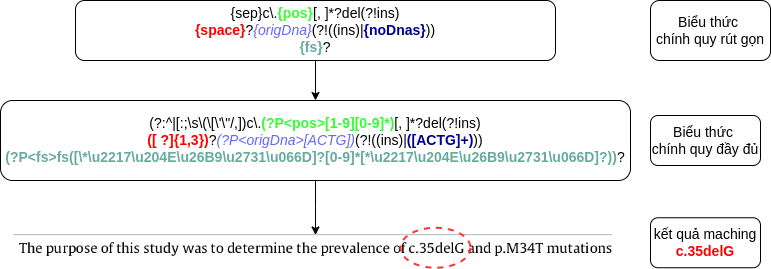
\includegraphics[width=1.1\linewidth]{Hinh_ve/regex.png}
\caption{Áp dụng biểu thức chính quy tìm kiếm mô tả biến thể đột biến}
\label{fig:poppler}
\end{figure}

\end{document}

